%%%%%%%%%%%%%%%%%%%%%%%%%%%HEADER%%%%%%%%%%%%%%%%%%%%%%%%%%%%%%
%%%%%%%%%%%%%%%%%%%%%%%%%%%HEADER%%%%%%%%%%%%%%%%%%%%%%%%%%%%%%
%%%%%%%%%%%%%%%%%%%%%%%%%%%HEADER%%%%%%%%%%%%%%%%%%%%%%%%%%%%%%
%Note: All the options like chapterprefix, pointednumbers, etc affect the way things are represented in the header of each page
\documentclass[a4paper,12pt,oneside,pointednumbers,bibtotoc,bigheadings,liststotoc]{scrbook}
% note that the expression "numbers=noenddot" remoes the dot after the number in figure captions
% for details see https://tex.stackexchange.com/questions/27250/remove-dot-after-number-in-figure-captions-while-keeping-the-dot-in-chapter-sect
\usepackage[utf8]{inputenc} %für Umlaute etc.
\usepackage[T1]{fontenc}
\usepackage[ngerman, english]{babel} %English titles (figure, table) und englische Silbentrennung
\usepackage{a4wide}
\usepackage{parskip} %see https://golatex.de/wiki/%5Cparskip to know what the package can do
\usepackage[pdftex]{color}
\usepackage{lmodern} \normalfont %to load T1lmr.fd  %weniger verpixelte Schrift; mehr Infos: http://www.namsu.de/Extra/pakete/Lmodern.html
%den genauen Trick für die untere Zeile kann ich hier nochmal nachlesen: http://tex.stackexchange.com/questions/22240/choosing-font-for-bold-small-caps-or-any-other-particular-familyseriesshape-c
\DeclareFontShape{T1}{lmr}{bx}{sc} { <-> ssub * cmr/bx/sc }{} 
\usepackage{a4} %anscheinend besser hier die Formatierung a4 wählen als als Option von documentclass
\usepackage[colorlinks = true,
		     bookmarks, 
		     linkcolor = red,
		     urlcolor = blue]{hyperref}
%\usepackage{fancyhdr}
\usepackage[right]{eurosym}
% the below two lines of code are necessary to make sure that the numbering of figures starts at 1 and then proceeds in steps of 1 instead of floating point numbers etc.
\usepackage{chngcntr}
\counterwithout{figure}{chapter}
\counterwithout{table}{chapter}
% the below code allows the adjustment 

\usepackage{amsmath, amssymb, amstext} %für Mathematik
\usepackage{mathstyle} %mehr Infos: http://www.ctan.org/pkg/mathstyle
\usepackage{blindtext} %to be able to place blindtext at certain locations
\usepackage[left=35mm, right=35mm, top=50mm, bottom=30mm]{geometry}%Seitenränder anpassen
\usepackage[onehalfspacing]{setspace} %1.5 Zeilgenabstand
\usepackage[round, comma]{natbib} %für die Bibliographie
%all four of the below packages are included for table creation
\usepackage{booktabs} 
\usepackage{array}
\usepackage{multirow}
\usepackage{tabularx}
\usepackage{lscape}
\usepackage{mathstyle} %mehr Infos: http://www.ctan.org/pkg/mathstyle
\usepackage[pdftex]{graphicx} %to include graphics
\usepackage{microtype} % makes pdf look better
\usepackage{booktabs}
%the below package allows the modification of the enumeration symbols
\usepackage{enumerate}% http://ctan.org/pkg/enumerate
\usepackage{dcolumn} % Ausrichtung nach Dezimalpunkt in Tabellen
\newcolumntype{.}{D{.}{.}{-1}}
\usepackage{setspace}
\pagestyle{headings}
% the below code is necessary to be able to customize the font of the Figure caption for figures
\usepackage{caption} % see https://www.namsu.de/Extra/pakete/Caption.html for more information!
\captionsetup[table]{font=scriptsize,labelfont=footnotesize,labelfont=bf, singlelinecheck = false, format=hang, justification=centering}
\captionsetup[figure]{font=scriptsize,labelfont=footnotesize,labelfont=bf, singlelinecheck = false, format=hang, justification=raggedright}%width=\dimexpr\textwidth-2cm\relax}
%\setlength{\textwidth}{15cm}
%\setlength{\textheight}{22.5cm}
%\setlength{\oddsidemargin}{1cm}
%\setlength{\evensidemargin}{0cm}
% \renewcommand{\baselinestretch}{1.2}
% \parskip1ex plus0.5ex minus0.5ex
%um die Überschriften im Inhaltsverzeichnis anzupassen
\usepackage{tocloft}
\renewcommand{\cftchapaftersnum}{.} %add period after the chapter number in ToC
% see https://tex.stackexchange.com/questions/411708/add-period-in-list-of-figures-list-of-tables
\renewcommand{\cftfigaftersnum}{.} %add period after figure number in list of figures
\renewcommand{\cfttabaftersnum}{.} %add period after table number in list of tables
\renewcommand\cftchapfont{\large\bfseries}%changes font and fontsize of chapters in toc
%\renewcommand\cftsecfont{\normalsize}
\renewcommand{\cfttoctitlefont}{\huge\bfseries}	%changes font of 'Content' header before toc
\renewcommand{\cftloftitlefont}{\huge\bfseries} %changes font of 'List of Figures'
\renewcommand{\cftlottitlefont}{\huge\bfseries} %changes font of 'List of Tables'
% the below commands move the beginning of toc, list of figures and list of tables further down 
% the page
\renewcommand\cftbeforetoctitleskip{2.7cm}
\renewcommand\cftbeforeloftitleskip{2.7cm}
\renewcommand\cftbeforelottitleskip{2.7cm}
%um die Überschriften im Text anzupassen
\usepackage{titlesec}
%der folgende Befehl ändert die Schriftart des "chapter"-Befehls
\titleformat{\chapter}{\large\bfseries\filright}{\Huge\thechapter.}{15pt}{\Huge}
\titleformat*{\section}{\large\bfseries}
\titleformat*{\subsection}{\normalsize\bfseries}
\titleformat*{\subsubsection}{\large\bfseries}
\titleformat*{\paragraph}{\small\bfseries}
% the below command is used to adjust the font-size of in-text block quotations
\usepackage{lipsum}% http://ctan.org/pkg/lipsum
\renewenvironment{quote}
               {\list{}{\rightmargin\leftmargin}%
                \item\relax\scriptsize\textquotedblleft\ignorespaces}
               {\unskip\unskip\textquotedblright\endlist}

%---------------------------------------------------------------------- Customizations ---------------------------------------------------------------------
%--------------------------------
%--------------------------------the entire below part is necessary to be able to include an abstract with the books document class
%--------------------------------
\usepackage{lipsum}
\newcommand\abstractname{Abstract}  %%% here
\makeatletter
\if@titlepage
  \newenvironment{abstract}{%
      \titlepage
      \null\vfil
      \@beginparpenalty\@lowpenalty
      \begin{center}%
        \bfseries \abstractname
        \@endparpenalty\@M
      \end{center}}%
     {\par\vfil\null\endtitlepage}
\else
  \newenvironment{abstract}{%
      \if@twocolumn
        \section*{\abstractname}%
      \else
        \small
        \begin{center}%
          {\bfseries \abstractname\vspace{-.5em}\vspace{\z@}}%
        \end{center}%
        \quotation
      \fi}
      {\if@twocolumn\else\endquotation\fi}
\fi
\makeatother

%--------------------------------
%--------------------------------the entire below part is necessary to be able to customize the header
%--------------------------------

\usepackage{fancyhdr} %Paket für Kopf- und Fußzeile laden
\setlength{\headheight}{15.2pt}
\pagestyle{fancy} %wir aktivieren unseren eigenen Seitenstil
%der folgende Befehl ändert die Schriftart im Header:
\renewcommand{\chaptermark}[1]{\markboth{\chaptername\  
\thechapter. \textit{#1}}{}}
\fancyhf{} %alle Kopf- und Fußzeilenfelder bereinigen
\fancyhead[R]{\thepage}
\fancyhead[L]{\rightmark}
\renewcommand{\headrulewidth}{0.4pt} %customizing obere Trennlinie

%% a bunch of code to control the length of the headrule
%% Length to control the \fancyheadoffset and the calculation of \headline
%% simultaneously
%\newlength\FHoffset
%\setlength\FHoffset{0cm}
%
%\addtolength\headwidth{2\FHoffset}
%
%\fancyheadoffset{\FHoffset}
%
%% these lengths will control the headrule trimming to the left and right 
%\newlength\FHleft
%\newlength\FHright
%
%% here the trimmings are controlled by the user
%\setlength\FHleft{0cm}
%\setlength\FHright{0cm}
%
%% The new definition of headrule that will take into acount the trimming(s)
%\newbox\FHline
%\setbox\FHline=\hbox{\hsize=\paperwidth%
%  \hspace*{\FHleft}%
%  \rule{\dimexpr\headwidth-\FHleft-\FHright\relax}{\headrulewidth}\hspace*{\FHright}%
%}
%\renewcommand\headrule{\vskip-.7\baselineskip\copy\FHline}
%% above is a bunch of code to control the length of the headrule

% the below code creates the opportunity to include a quote at the beginning of a chapter
% customize chapter format:
\KOMAoption{headings}{twolinechapter}
\renewcommand*\chapterformat{\thechapter\autodot}

% add chapter quote to beginning of chatpers
% see https://tex.stackexchange.com/questions/53377/inspirational-quote-at-start-of-chapter
\makeatletter
\renewcommand{\@chapapp}{}% Not necessary...
\newenvironment{chapquote}[2][2em]
  {\setlength{\@tempdima}{#1}%
   \def\chapquote@author{#2}%
   \parshape 1 \@tempdima \dimexpr\textwidth-2\@tempdima\relax%
   \itshape}
  {\par\normalfont\hfill--\ \chapquote@author\hspace*{\@tempdima}\par\bigskip}
\makeatother

\newcommand\textbox[1]{%
  \parbox{.333\textwidth}{#1}%
}

%--------------------------------
%--------------------------------additional customizations
%--------------------------------
\setlength{\parindent}{0pt} %legt die Einrücktiefe der ersten Zeile für alle folgenden Absätze fest
% adds a command for exceptional paragraph identation!
\newcommand{\forceindent}{\leavevmode{\parindent=1em\indent}}
\setlength{\abovecaptionskip}{-15pt plus 3pt minus 2pt} %modify vertical space between figure and caption
\renewcommand*{\paragraph}[1]{\subsubsection*{#1} \vspace{-3mm}} %mit diesem Befehl kann man ganz einfach
%PARAGRAPH eingeben und latex macht sofort eine subsubsection ohne Nummerierung usw draus
%customizations für Vektoren (dass sie bold dargestellt werden anstatt mit einem Vektorpfeil)
\let\oldhat\hat
\renewcommand{\vec}[1]{\boldsymbol{#1}}
\renewcommand{\hat}[1]{\oldhat{\boldsymbol{#1}}}


%%%%%%%%%%%%%%%%%%%%BEGINNING OF THE DOCUMENT%%%%%%%%%%%%%%%%%%%%%%%%
%%%%%%%%%%%%%%%%%%%%BEGINNING OF THE DOCUMENT%%%%%%%%%%%%%%%%%%%%%%%%
%%%%%%%%%%%%%%%%%%%%BEGINNING OF THE DOCUMENT%%%%%%%%%%%%%%%%%%%%%%%%
\begin{document}
%----------------------------------------------------------- Beginn Titelseite -------------------------------------------------------------------------------
%\changefont{ppl}{m}{n} %mit diesem Befehl kann global ganz leicht die Schriftart geändert werden
\newgeometry{left=30mm, right=30mm, top=0mm, bottom=0mm}
\begin{titlepage}
    \begin{center}
        \hspace*{-0.27\textwidth}
\includegraphics[width=1.419\textwidth, trim = 5mm 250mm 0mm 0mm, clip = TRUE]{logo.pdf}\hspace*{-0.3\textwidth}
        \quad \\[0mm]
        \newcommand{\HRule}{\rule{\linewidth}{0.3mm}} %Befehl zum Erstellen der Linie
        \HRule \\[-1mm]
        \Huge{\scshape\bfseries Time-Varying Uncertainty and Business Cycles} \\[-5mm]
        \HRule \\[2mm]
        \large {\scshape An Inquiry into the Measurement of Uncertainty and its\\
        				Macroeconomic Effects Using the Example of the US} \\[10mm]
        \large Master's Thesis \\[10mm]
        \large in partial fulfillment of the requirements \\for the degree of Master of Science (M.Sc.)\\
                  in Applied Economics \\[10mm]
                  
        submitted to\\
        Univ.-Prof. Dr. Johann Scharler \\[10mm]
        Department of Economics\\
        Faculty of Economics and Statistics\\
        Leopold-Franzens-Universität Innsbruck \\[10mm]
        by \\ Mag. Marcel A. Kropp \\[10mm]
        Innsbruck, July 2018
    \end{center}
\end{titlepage}
%----------------------------------------------------------- Ende Titelseite -------------------------------------------------------------------------------
\restoregeometry

%----------------------------------------------------------- Beginn Widmung Mum ---------------------------------------------------------------------
%Kurze Widmung an Mum.
\thispagestyle{empty} %bewirkt, dass die Striche oben wegfallen und, dass die Seitenzahl wegfällt.
\null\vspace{\stretch{1}}
    \begin{flushright}
       \large \textit{To my Mum.}\\
    \end{flushright}
\vspace{\stretch{2}}\null
%----------------------------------------------------------- Ende Widmung Mum ------------------------------------------------------------------------


%----------------------------------------------------------- Beginn Widmung Alle ------------------------------------------------------------------------
\newpage
\pagestyle{empty} %bewirk, dass die Striche oben wegfallen und, dass die Seitenzahl wegfällt.
What I have written five years ago still holds more than ever:\\
My family has been my strongest support in all my life. I especially want to express my gratitude to my dear uncle Dr. med. Farshid Mavaddat, my cousins Dr. Paik Saber and Neisan Saber and my aunt Mahshid Mavaddat.\\
Most of all I want to thank my Mum, Dorrie Mavaddat, who has always been there for me and supported and helped my in all my ventures. It is due to her that I stand where I am today.
    \begin{flushright}
         Innsbruck, July 2018\\
    \end{flushright}
\pagestyle{headings}
%-------------------------------------------------------------- Ende Widmung Alle ------------------------------------------------------------------------

%\clearpage
%\setlength{\hoffset}{0mm}

%jetzt kommen die abstracts auf Englisch und Deutsch
\thispagestyle{empty} 
%\quad \\[2cm]
\selectlanguage{english}
\begin{abstract}
\blindtext
\end{abstract}

%\quad \\[10mm]
\begin{otherlanguage}{ngerman}
\begin{abstract}
\blindtext
\end{abstract}
\end{otherlanguage}


\restoregeometry

\thispagestyle{empty}
\pagestyle{fancy} %bewirkt, dass die Striche oben wieder dazukommen
\pagenumbering{roman} %bewirkt, dass LateX i, ii, usw zählt
\setcounter{page}{7} %und aber schon bei 7 anfängt zu zählen
%\renewcommand{\contentsname}{Table of Contents}
%\renewcommand{\cftdot}{\ensuremath{\ast}} %\ensuremath{\ast} does sth funny to the dots in the toc
\tableofcontents
\newpage
\listoffigures

\newpage
\listoftables

\newpage

%%%%%%%%%%%%%%%%%AB HIER BEGINNT DER INHALT DER ARBEIT%%%%%%%%%%%%%%%%%%%%%
%%%%%%%%%%%%%%%%%AB HIER BEGINNT DER INHALT DER ARBEIT%%%%%%%%%%%%%%%%%%%%%
%%%%%%%%%%%%%%%%%AB HIER BEGINNT DER INHALT DER ARBEIT%%%%%%%%%%%%%%%%%%%%%
\pagenumbering{arabic} %mit diesem Befehl wechseln wir auf 1, 2, 3, usw. zum zählen.


%%%%%%%%%%%%%%%%%%%%%%%%%%%%%%%%%%%%%%%%%%%%%%%%%%%%%%%%%%
%%%%%%%%%%%%%%%%%%%%%%%%%%%%%%%%%%%%%%%%%%%%%%%%%%%%%%%%%%
%%%%%%%%%%%%%%%%%%%%%%%%%%%%%%%%%%%%%%%%%%%%%%%%%%%%%%%%%%
%%%%%%%%%%%%%%%%%%%%%%%%%%%%%%%%%%%%%%%%%%%%%%%%%%%%%%%%%%
\chapter{Introduction}
% the below code making use of "begingroup" etc. is only necessary if I want to customize the font for a particular part of the thesis
%\begingroup
%\fontsize{10pt}{12pt}\selectfont
It can be commonly postulated that being faced with uncertainty is a state inherent to life's existence and in every aspect a natural part of our complex world. \\
Focussing on \textit{economic} uncertainty, \href{http://citeseerx.ist.psu.edu/viewdoc/download?doi=10.1.1.334.4248&rep=rep1&type=pdf}{an investor being concerned about the performance of her assets, an employee being worried about future income streams during retirement or at all still having a job one year from now or a business continuously defending its position on the market are just a few examples} of individuals or a collective being exposed to uncertainty in every-day life. Many of these risks/uncertainties\footnote{Note that we are currently still using these terms interchangeably but will give a brief overview of the discussion and their subtle differences in the literature below.} have given rise to institutions and entire industries as an integral part of today's modern economies: sophisticated financial markets (with their risk-transformation-function being a pivotal element besides the purpose to raise capital) and the finance and insurance industry would not exist (or albeit in a different form) if it was not for the existence of uncertainty. On the academic front, ever more complex models promise remedy to make exposures to uncertainty and foresight calculable and/or manageable.\\
\\
But which specific events can cause (economic or political) uncertainty that ultimately feed  into the micro-level giving rise to exemplary scenarios we just discussed?\\
\href{https://site.stanford.edu/2018/session-6}{On an aggregate level, as aptly formulated by Nicholas Bloom}\footnote{Bloom is part of a larger group of contributors to the most recent macroeconomic literature that has started to systematically disentangle the effects of uncertainty both theoretically and empirically.}, after the Great Recession and the subsequent turmoil in the Eurozone's sovereign debt markets and the Arab Spring being just a few examples, the most recent major political events\footnote{One could potentially also call them 'shocks'.} of Brexit, Trump's election in the US,  and a seeming intensification of tensions between forces of the West and East have brought uncertainty into the spotlight again suggesting that alleged 'tail-events' are far from improbable.\\
\\
On a high level, \citet{dequesh:00} identifies four basic social practices in today's societies that have a stabilizing effect on the coexistence in our (as  he calls it) \textit{economic reality}: (1) legal contracts (that reduce the uncertainty of future values of nominal variables), (2) the 'State' which enforces legal contracts in case one party to a contract would decide to not fulfill its obligations, (3) Market-Makers (a very prominent example being central banks in their roles as lenders of last resort), and lastly, (4) informal institutions including conventions like 'socially shared and/or prescribed standards of thought and behavior'. \\
Together these features improve subjective and objective uncertainty but can obviously not completely eliminate it. \\
\\
Although we do not want to roll up the subject from a philosophical (or even religious) perspective, whoever analyses \textit{uncertainty} and its underlying meaning in the literature hoping to clearly differentiate it from related concepts such as \textit{risk} or \textit{ambiguity}, will quickly realize that an unambiguous definition is not straightforward. Confining ourselves to economics only, there is a vast array of literature starting at the beginning of the 20th century that refers to these concepts in different schools of thought that at their core do have a philosophical component to them. Different parlance within the profession which \href{http://www.economics-ejournal.org/economics/discussionpapers/2015-36/file}{even causes similar concepts to be named differently} or the same term being used with a different meaning additionally complicates matters.\\
\\
While a thorough discussion of every aspect of the related concepts is beyond the scope of this work, we still want to give a brief overview of a few insights by referring to a few selecting writings:\\
\forceindent \citet{dow:16} tries to clarify the difference between the mainstream and Keynesian\footnote{Keynes and Knight are often-times regarded as the two prominent figures that introduced the concept of \textit{fundamental uncertainty} into the economic sciences.} understanding of \textit{uncertainty}\footnote{\citet{dow:16} also makes account to von Mises, Hayek and Shackle who have also dealt with uncertainty in their works but focusses on Keynes's views on fundamental uncertainty arguing for it to be the most developed and philosophically-grounded counterpoint to the mainstream theory.}, its distinction from \textit{risk} and the resulting theoretical implications\footnote{Note that there are also schools that reject the distinction between \textit{uncertainty} and \textit{risk} altogether (e.g., \citealp{savage:54}).}. According to her assessment, in the traditional mainstream analysis within a Bayesian framework most knowledge is viewed as known or known to be stochastic in some form (called \textit{risk}), meaning that the state space is known and numerical probabilities can be assigned. Under this approach, mainstream traditional macroeconomic models give only very limited room, if any, to \textit{uncertainty} as a state of absence of such probabilities in the form of exogenous sources of shocks\footnote{\citet[p. 43]{dequesh:00} refers to some economists partly neglecting fundamental uncertainty following the argument that it might lead to 'theoretical nihilism' (see e.g., \citealp{coddington:82}).}. \\
Read from this dualistic mainstream perspective, \citet{dow:16} asserts that Keynes's standpoint was also for a long time interpreted in a dualistic way, albeit flipped in the sense that only in special circumstances, knowledge (here referred to as \textit{risk}) could be treated as certain and (fundamental) uncertainty was regarded as the general case (see the introduction in \citealp{keynes:21}). This dualistic interpretation was reinforced by Keynes's reflections on long-term expectations~\citep[p. 214/214]{keynes:37}: 
``About [uncertainty] there is no scientific basis on which to form any calculable probability whatever. We simply do not know.''\\
\\
But \citet{dow:16} clarifies that in the meantime it is well-established that Keynes did not give up on scientific knowledge (i.e., did not advocate nihilism) by giving so much weight to uncertainty but that his view on uncertainty is rather multidimensional and consists of various degrees. As an advocate of this view, \citet{dequesh:00} argues that Keynes referred to both ambiguity in his early writings (\citealp{keynes:21})\footnote{According to interpreters, in terms of \citet{keynes:21}, for both ambiguity and fundamental uncertainty there is no basis for the assignment of point, numerical probabilities \citep{dequesh:00}.} and fundamental uncertainty in his later ones (\citealp{keynes:37}) and that simply speaking of Keynesian uncertainty may actually be too vague in most circumstances. \\
\\
\citet[p. 330]{camererandweber:92} describe ambiguity as ``uncertainty about probability, created by missing information that is relevant and could be known''. \citet[p. 623]{dequech:14} states that while usually the decision-maker under ambiguity cannot reliably assess the probability of each event, she usually knows all possible events (or it is at least ``predetermined or knowable ex ante``) while the case of fundamental uncertainty ``[...] is characterized by the possibility of creativity and non-predetermined structural change''. So under this concept and ``[w]ithin the bounds imposed by natural laws, the list of possible events is not predetermined or knowable ex ante [...] as \textit{the future is yet to be created}\footnote{Italics added.}'' \citep[p. 623]{dequech:14}. \citet{dequesh:00} sees the work of \citet{shackle:72} as advocating this argument.\\
\\
With regard to fundamental uncertainty, \citet{dequesh:00} mentions technological or managerial innovations as examples of human creativity that can disrupt our realities which is closely connected to the process of creative destruction of \citet{schumpeter:42}. Unpredictable structural changes (e.g. historical changes) to our economic reality on the other hand are more typically political, social or cultural disruptions where institutions and technological change play a key-role. Interestingly, the capitalist system as we know it is regarded as endogenously causing uncertainty due to competing economic actors and decision-makers innovating in search for extra profits (see \citealp{kregel:87})\footnote{Despite of the above remarks, Keynes' notion of uncertainty as described in \citet{keynes:21} and its connection to \citet{keynes:37} has been subject to much controversy due to differing interpretations \citep{dequesh:00}.}.\\
\\
Coming back to the mainstream view, while the crisis and subsequent Great Recession has triggered a rethinking of the mainstream approach to uncertainty by emphasizing ``institutional impediments to information access (asymmetric information)'' \citep[p. 8]{dow:16}, degrees of uncertainty were only gradually added to the picture: the term 'ambiguity' was acquired as well (also following \citealp[p. 330]{camererandweber:92}) to account for these various degrees of uncertainty while 'unknown unknowns' (i.e. unimaginable events or 'black swans' as dubbed by \citealp{taleb:08}) would have to be seen as \textit{'knowable unknowns'} to still be consistent with the Bayesian framework. The term 'ambiguity' is thereby introduced as falling either into the category of risk or uncertainty depending on the ability to quantify higher-order probabilities.
\\
\\
Trying to establish a typology within the introduced terms, \citet{dequech:14}  sets up three dimensions along which he classifies relevant concepts\footnote{Apart from this classification we do not discuss any further interrelationships between the various concepts.}: 
\begin{enumerate}
	\item between substantive and procedural uncertainty:\footnote{Proposed by \citet[p. 145]{dosiandegidi:91} whereby substantive uncertainty results from the ``lack of all the information which would be necessary to make decisions with certain outcomes'' and procedural uncertainty from ``limitations on the computational cognitive capabilities of the [respective] agents to pursue unambiguously their objectives, given [...] available information'' in a complex decision problem. }
	\item between weak and strong uncertainty:\footnote{Whereby under weak uncertainty ``[...] an agent can form [...] a unique, additive and fully reliable probability distribution'' based on relevant and good-quality information and strong uncertainty consequently ``[...] by the absence of such a distribution'' \citep[p. 622/623]{dequech:14}.} \\
	weak uncertainty is then further subdivided into \textit{Knightian risk} (see \citet{knight:21}; often simply called 'situations of risk' where agents are faced with objective probabilities, either a priori or statistical probabilities (i.e., relative frequencies) and \textit{Savage's uncertainty} (see \citet{savage:54}; who introduced a full theory of 'personal probability' where \textit{personal} belief governs probabilities, based on prior \href{https://archive.org/stream/in.ernet.dli.2015.223806/2015.223806.The-Foundations#page/n289/mode/2up}{groundbreaking work of} \href{http://www.brunodefinetti.it/Link/Subjective%20Expected%20Utility%20-%20Intro.htm}{\citet{ramsey:26}\footnote{Written ``in opposition'' to \citet{keynes:21}.} and \citet{finetti:37}});
	\item between ambiguity and fundamental uncertainty.\footnote{Which are two types of strong and substantive uncertainty \citep{dequesh:00}.}
\end{enumerate}
\vspace{1cm}


Abstracting from the (philosophical) considerations above, is there any consent in the literature about whether uncertainty can be quantified and, if so, how this could be achieved? And once having a meaningful measure of unertainty, what \textit{real} effect, if any, does it exert on business cycles? \\
\\
Within the past ten years and largely triggered by a seminal work by \citet{bloom:09}\footnote{Bloom's contribution triggered a wave of studies that challenged the effects that he had reported in his initial publication in \citet{bloom:09}.}, macroeconomists have intensively started studying this question more intensively than ever before. At a first glance, as summarized by \citet[p. 1177]{juradoetal:15}, partial equilibrium analyses to date suggest that increased levels of uncertainty ``[...] can depress hiring, investment, or consumption if agents are subject to fixed costs or partial irreversibilities (a 'real options' effect), if agents are risk averse (a 'precautionary savings' effect), or if financial constraints tighten in response to higher uncertainty (a 'financial frictions' effect).'' \\
\\
While these effects have been identified by and large in the literature, the timing, extent and causality of effects remain hotly debated not least because of various uncertainty measures being used that try to quantify a decisive factor: unobservable, time-varying aggregate economic uncertainty.
\\
\\
The remainder of this thesis is organized as follows. Section~\ref{MeasuringUncertaintyandaHistoricalView} explores alternative uncertainty measures, their time-series properties as well as some 'stylized facts' on uncertainty, Section~\ref{UncertaintyandBusinessCyclesRelatedLiterature} briefly reviews the related literature triggered by the seminal work of \citet{bloom:09}, Section~\ref{sec:EmpiricalAnalysis} is dedicated to the empirical analysis using data for the US and starting from a replication of the benchmark model of \citet{bloom:09} contrasts the isolated effects based on various uncertainty measures, samples and estimation techniques (VARs and the local projection method following \citealp{jorda:05}), and Section~\ref{Conclusion} summarizes and concludes. \\
Additional details and results are outsourced to Appendix~\ref{DataAndCode} including information on the data and the entire code and Appendix~\ref{VARAndLocalProjection} including information on the differences between VARs and the local projection method by \citet{jorda:05}.








%%%%%%%%%%%%%%%%%%%%%%%%%%%%%%%%%%%%%%%%%%%%%%%%%%%%%%%%%%
%%%%%%%%%%%%%%%%%%%%%%%%%%%%%%%%%%%%%%%%%%%%%%%%%%%%%%%%%%
%%%%%%%%%%%%%%%%%%%%%%%%%%%%%%%%%%%%%%%%%%%%%%%%%%%%%%%%%%
\chapter{A Closer Look At Uncertainty}
\label{MeasuringUncertaintyandaHistoricalView}

\begingroup
    \fontsize{8pt}{12pt}\selectfont
    Note to self:
\begin{itemize}
	\item  The IMF Working Paper (Measuring Global and Country-Specific Uncertainty) is a very helpful resource because the introduction to their paper is very insightful with lots of useful information about the current state of research in this respect!
\end{itemize}
\endgroup


As mentioned in the Introduction above, studies that try to explain the impact of uncertainty, if any, on aggregate economic fluctuations\footnote{Note that Section~\ref{UncertaintyandBusinessCyclesRelatedLiterature} will review these studies in more detail.} not only differ with respect to econometric specifications (which we will examine in Section~\ref{sec:EmpiricalAnalysis}) but also to the deployed \textit{uncertainty measure} itself. In fact, there is currently a very active and dedicated branch of the literature that tries to answer that one question: How can we best and most objectively measure uncertainty? And out of the suggested uncertainty measures to date, which one is the preferred one?\\
\\
In what follows below we, first, want to review a selection\footnote{We have decided to restrain ourselves to \textit{four} measures which are among the most commented-on in the literature and which we examine in more detail for the purpose of this thesis.} of uncertainty measures that have been used/suggested in the literature to date including their pros and cons and, second, investigate some of their time series properties to get a feeling of their similarities as well as discrepancies.

\section{Measuring Uncertainty}
\label{sec:MeasuringUncertainty}
Various uncertainty measures exist (and not \textit{the one} measure) because the stochastic process which we commonly call 'uncertainty' is unobservable. \citet[p. 1182]{juradoetal:15} emphasize that ``[t]he literature on measuring uncertainty is still in its infancy'' and so far existing research has popularized various proxies or indicators of uncertainty.

The lack of an objective uncertainty measure hence poses a serious challenge to studies trying to quantify its macroeconomic effects: they have to come up with a reasonable uncertainty measure in the first place. \citet[p. 1178]{juradoetal:15} explain that ``[w]hile most of the [above mentioned] measures have the advantage of being directly observable, their adequacy as proxies for uncertainty depends on how strongly they are correlated with this latent stochastic process [i.e., with unobservable uncertainty]''.\\
\\ 
Besides creating their own measure of economic uncertainty, \citet{orlikandveldkamp:14} describe commonly used proxies of uncertainty by means of the following taxonomy and refer to selected works along the way\footnote{Note that we have slightly extended the original taxonomy of \citet{orlikandveldkamp:14} by mixing it with \citet{bontempietal:16}'s taxonomy. Only the measures that link to a dedicated section will examined in more detail below.}:
\begin{itemize}
	\item \textbf{Forecast Dispersion:} add detailed description!
	\item \textbf{Mean-Squared Forecast Error:} add detailed description!
	\item \textbf{Volatility and Confidence Measures}, where we find three alternative approaches:
		\begin{itemize}
			\item 'finance-based' - measures, assuming that financial volatility is a suitable indicator for aggregate macroeconomic uncertainty: 
			\begin{itemize}
				\item the traditional measure of uncertainty is the implied (e.g., the market volatility indices VIX/VXO) or realized volatility of stock market returns; based on these measures, \citet{bloom:09} constructs his shock-measure (henceforth called 'Bloom-shock'; see Section~\ref{sec:bloomshock} below)
			\end{itemize}
			\item 'forecast-based'\footnote{Note to self: we still have to fit 'the cross-sectional dispersion of firm profits, stock returns, or productivity' somewhere into our taxonomy!} - measures that rely on both an economy's predictability and the measurement of discrepancies between professional forecasts assuming that impeded predictability and a large dispersion between forecasts points at a more uncertain economy:
			\begin{itemize}
				\item cross-sectional dispersion measures of subjective business or consumer confidence (forecasts) based on survey data: e.g., \citet{bachmannetal:13} use survey data in their analysis (note to self: briefly mention their used measures), \citet{juradoetal:15} also mention analysts' forecasts (as e.g., used by D'Amico and Orphanides); \citet{leducandliu:16} instead use a measure constructed using data from the Thomson Reuters/Uniersity of Michigan Surveys of Consumers (henceforth called MSoC-index; see Section~\ref{sec:michigansurvey} below)
				\item \citet{juradoetal:15} construct a (as \citet{orlikandveldkamp:14} call it) 'state-of-the-art' macro uncertainty index (henceforth called 'macro uncertainty index' see Section~\ref{sec:macrouncertainty})
			\end{itemize}
			\item 'news-based' - approaches that measure the degree of uncertainty by extracting the frequency with which specific words appear in newspaper articles, assuming that journalists are able to assess emerging uncertainty \footnote{Note that this approach is similar to the narrative analysis used by \citet{romerandromer:04}, \citet{romandrom:17} or \citet{ramey:09}.}: 
			\begin{itemize}
				\item \citet{alexopoulosandcohen:09} construct a news-based index derived from the number of New York Times' articles on uncertainty and economic activity,
				\item \citet{bakeretal:15} construct an index of economic policy uncertainty (EPU) for a number of countries (including the United States) by searching for uncertainty-related keywords within a pool of widely read country-specific newspapers (henceforth called 'EPU index'; see Section~\ref{sec:epuindex}),\\
			in a similar vein, \citet{moore:17} constructs an index of economic uncertainty for Australia,
				\item inspired by classical 'news-based' - approaches, \citet{bontempietal:16} and \citet{castelnuovoandtran:17} construct 'Google Trends Uncertainty' indices (they call their index GT- and GTU-index, respectively) based on freely accessible, real time Google Trends data (henceforth called BGS-index and CT-index, respectively; see Section~\ref{sec:googletrends}); thereby the focus is shifted from journalists drawing the public's attention to specific topics to the public's individual Internet searches
			\end{itemize}
		\end{itemize}
\end{itemize} 

We will discuss a few of these measures in turn.


\subsection{VXO/Bloom-shock: \citet{bloom:09}}
\label{sec:bloomshock}
\begingroup
    \fontsize{8pt}{12pt}\selectfont
    Note to self:
\begin{itemize}
	\item  \citet{bloom:09} describes the identification of shocks both in the Appendix (section A.1.2, p. 675;) as well as in the main text on p. 630. The explanation in the main text states:\\
``The main stock-market volatility indicator is constructed to take a value 1 for each of the shocks labelled in the figures above and a 0 otherwise. These shocks were explicitly chosen as those events \textit{when the peak of HP detrended volatility level rose significantly above the mean.} In particular, the threshold was 1.65 standard deviations above the mean, selected as the 5\% one-tailed significance level \textit{treating each month as an independent observation}.''
	\item I definitely have to take into account what Hans said: the construction of the Bloom-shock explicitly tries to argue that the shocks are exogenous by construction - here I should 
\end{itemize}
\endgroup


The construction of the 'Bloom-shock' as outlined in \citet{bloom:09} is performed in multiple steps and uses two data-sources\footnote{Note that in the original contribution of \citet{bloom:09} the data logically only ranges until 2009 while we now have almost 10 more years of VXO data at our disposal.}: (i) VXO-data from the Chicago Board Options Exchange (CBOE) for the period where data is available (i.e., 1986 - 2018)\footnote{The VXO - index (for details see the the homepage of the CBOE) reflects the market's expected implied volatility based on S\&P100 options 30 days to expiration and hence captures expected volatility of equity prices. Note that the VIX introduced as of 2003 instead is based on prices of S\&P500 options.} and (ii) actual monthly volatilities (for the period pre-1986) calculated as the monthly standard deviation of the daily S\&P500 index (normalized to the same mean and variance as the VXO index for when the two series overlap, i.e., from 1986 - 2003)\footnote{The R-Code replicating all the steps for the construction of the Bloom-shock is available in Appendix~\ref{sec:rcode}.}. The result is one continuous volatility measure as shown in Figure~\ref{fig:volatility}.\footnote{In the following we refer to this spliced version as the VXO index.}
\begin{figure}[!ht]
   \centering
   \setlength\fboxsep{0pt}
   \setlength\fboxrule{0pt}
   \fbox{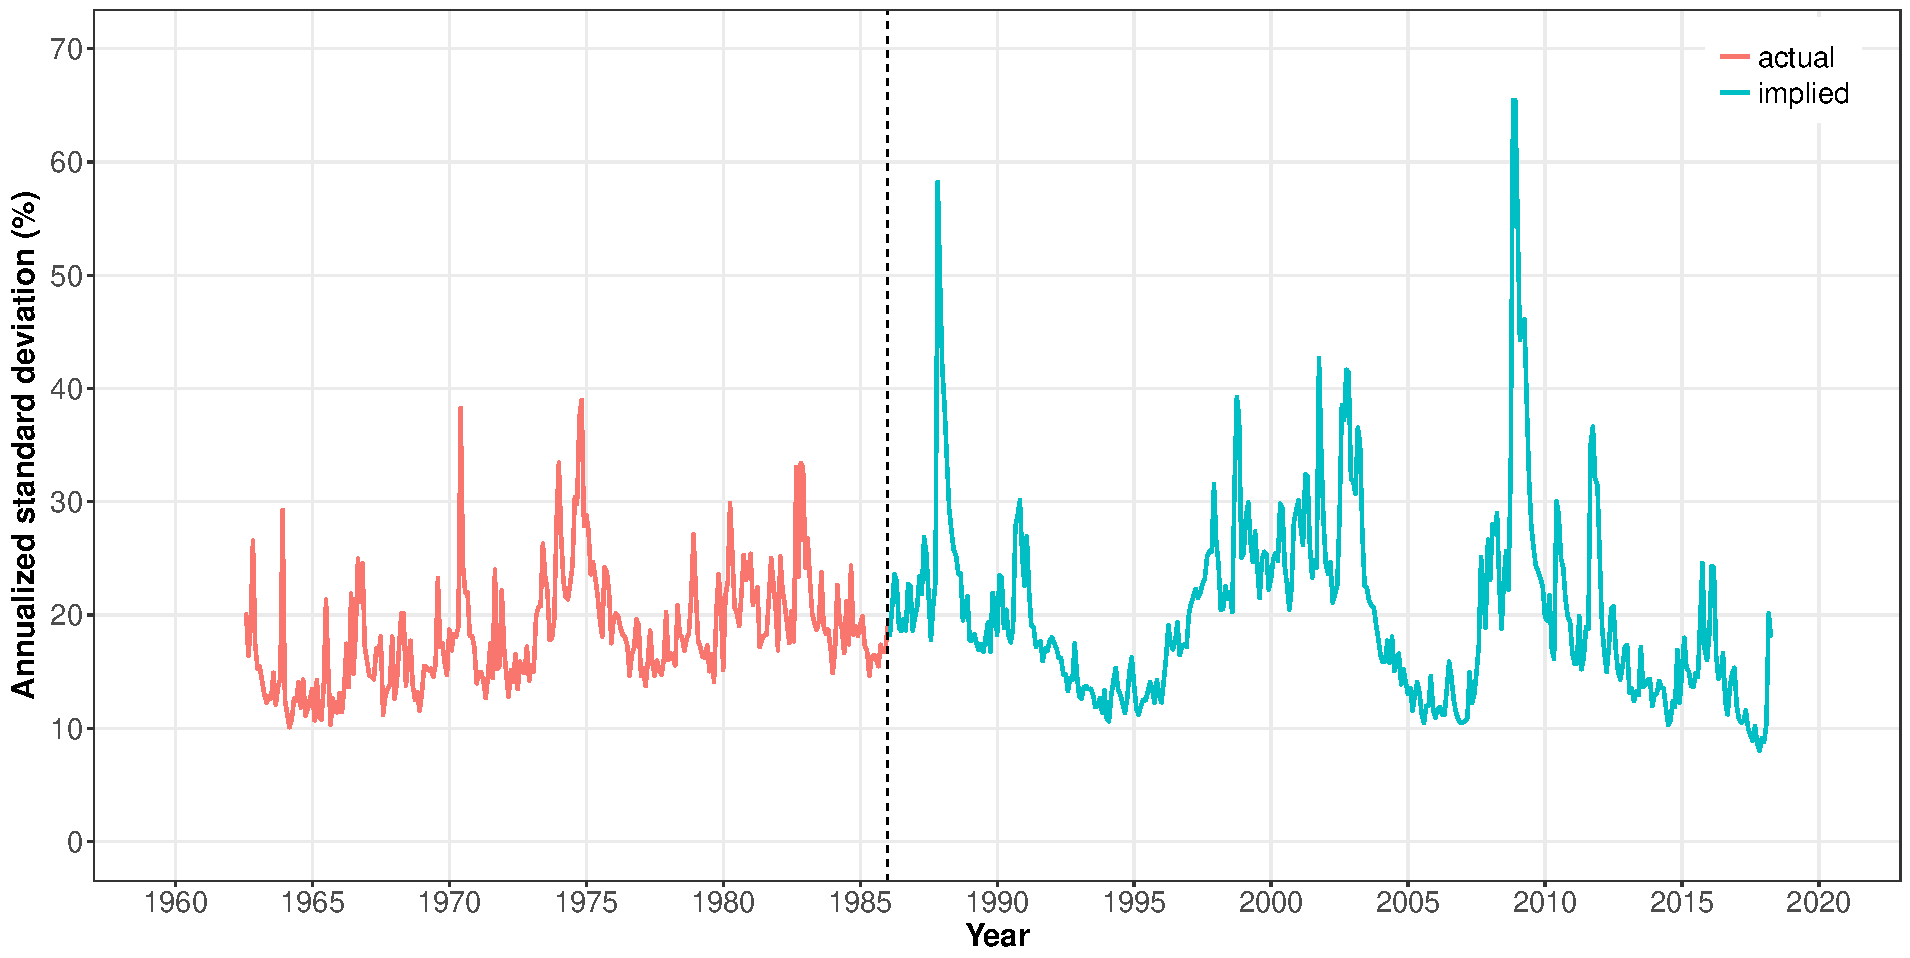
\includegraphics[trim=1cm -2.5cm 0.8cm -1cm, width=0.95\textwidth]{volatility.pdf}}
      \caption[Monthly U.S. stock market volatility.]{Monthly U.S. stock market volatility.
      \textit{Note:} From 1986 onwards CBOE VXO index of percentage implied volatility, on a hypothetical at the money S\&P100 option 30 days to expiration. Before 1986 actual monthly returns volatilities are calculated as the monthly standard deviation of the daily S\&P500 index normalized to the same mean and variance as the VXO index when they overlap from 1986 - 2003.}
   \label{fig:volatility}
\end{figure}

The derivation of the 'Bloom-shocks' (i.e., an indicator variable that takes a value of 1 for an event labelled as a 'shock') then works as follows:
\begin{enumerate}[i]
	\item detrend the volatility-measure from above (\citet{bloom:09} uses a HP-filter with $\lambda = 129,600$); 
	\item according to \citet{bloom:09}, the actual shocks are then chosen as those events with stock-market volatility more than 1.65 standard deviations above the HP-detrended mean (selected as the 5\% one-tailed significance level) of the stock-market volatility series; thereby each month is being treated as an independent observation
\end{enumerate}

\begin{figure}[!h]
   \centering
   \setlength\fboxsep{0pt}
   \setlength\fboxrule{0pt}
   \fbox{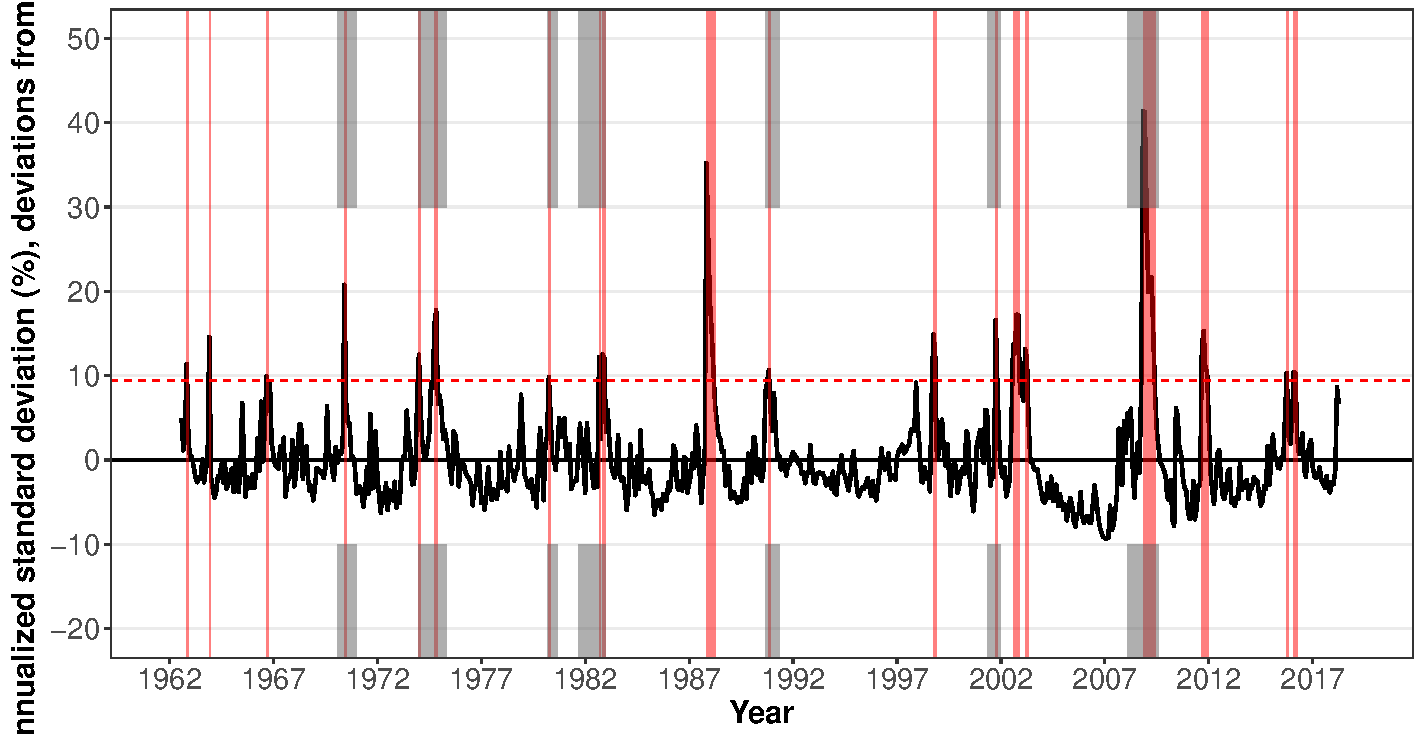
\includegraphics[trim=1cm -2.5cm 0.8cm -1cm, width=0.95\textwidth]{volatility_cycle_shocks2.pdf}}
      \caption[Monthly U.S. stock market volatility including Bloom-shocks and NBER recession dates.]{Monthly U.S. stock market volatility. Red shaded areas correspond to dates where volatility series exceeds 1.65 standard deviation above the series' mean. Grey shaded areas denote NBER recession dates in the US.}   \label{fig:volatility_cycle_shocks2}
\end{figure}

Ultimately, this results in identified 'shocks' as shown in Figure~\ref{fig:volatility_cycle_shocks2} where the shaded areas correspond to the 'Bloom-shock' being equal to $1$ (i.e., where the dashed horizontal line representing 1.65 standard deviations above the HP filtered mean crosses the detrended series). Accordingy, Table~\ref{tab:bloom_shocks} spells out the exact dates of the identified shocks including when the 'Bloom-shock' started (first column), when it ended (second column), the amount of consecutive months within a dedicated shock-period (third column), the date with the maximum volatility within the dedicated shock-period (fourth column) and the corresponding maximum volatility in the last column.
%\begin{figure}[hbt]
%   \centering
%   \setlength\fboxsep{0pt}
%   \setlength\fboxrule{0pt}
%   \fbox{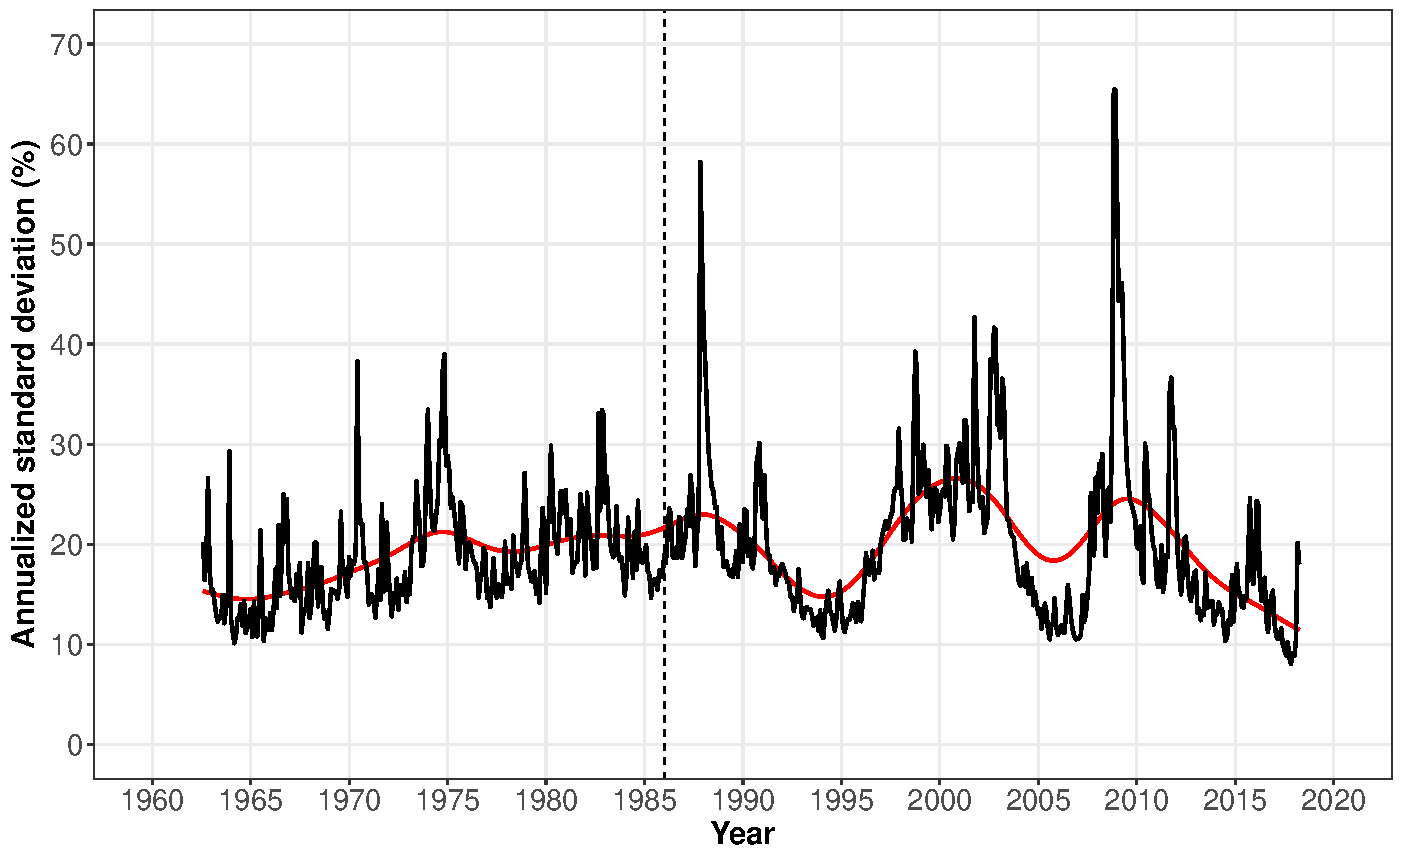
\includegraphics[trim=1cm -2.5cm 0.8cm -1cm, width=0.95\textwidth]{volatility_trend.pdf}}
%      \caption[Monthly U.S. stock market volatility and HP-filtered trend.]{Monthly U.S. stock market volatility and HP-filtered trend.
%      \textit{Note:} HP-filtered trend was calculated using a smoothing parameter $\lambda = 129,6000$.}   \label{fig:volatility_trend}
%\end{figure}


%\begin{figure}[h]
%   \centering
%   \setlength\fboxsep{0pt}
%   \setlength\fboxrule{0pt}
%   \fbox{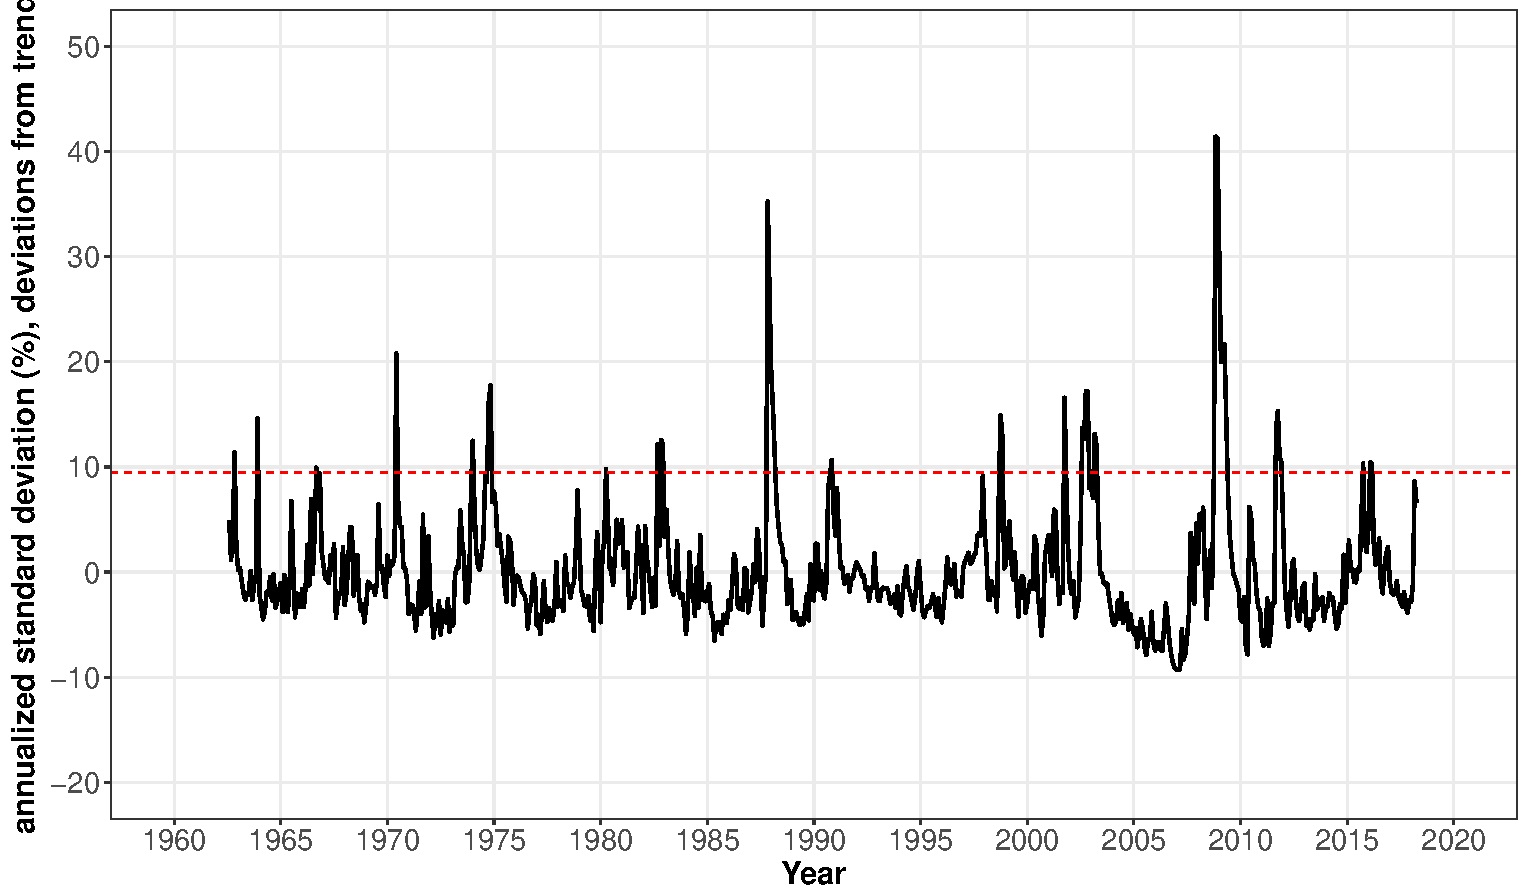
\includegraphics[trim=1cm -2.5cm 0.8cm -1cm, width=0.95\textwidth]{volatility_cycle_shocks.pdf}}
%      \caption[Monthly U.S. stock market volatility and HP-filtered trend.]{Monthly U.S. stock market volatility and HP-filtered trend.
%      \textit{Note:} HP-filtered trend was calculated using a smoothing parameter $\lambda = 129,6000$.}   \label{fig:volatility_cycle_shocks}
%\end{figure}



\begin{table}[htp] 
\begin{center}
\caption{Replication of shocks following \citet{bloom:09}.}
\scalebox{0.8}{
    \begin{tabular}{cccccc}
    \hline
         yearmon_start & yearmon_end & duration & yearmon_max & max_vol \\ \hline
        Nov 1962 & Nov 1962 & 1 months & Nov 1962 & 26.58\% \\
        Dec 1963 & Dec 1963 & 1 months & Dec 1963 & 29.28\% \\
        Sep 1966 & Sep 1966 & 1 months & Sep 1966 & 24.99\%\\
        Jun 1970 & Jun 1970 & 1 months & Jun 1970 & 38.27\% \\
        Jan 1974 & Jan 1974 & 1 months & Jan 1974 & 33.44\% \\
        Oct 1974 & Nov 1974 & 1 months & Nov 1974 & 38.98\% \\
        Apr 1980 & Apr 1980 & 1 months & Apr 1980 & 29.86\% \\
        Sep 1982 & Sep 1982 & 1 months & Sep 1982 & 33.05\% \\
        Nov 1982 & Dec 1982 & 2 months & Nov 1982 & 33.43\% \\
        Nov 1987 & Mar 1988 & 5 months & Nov 1987 & 58.22\% \\
        Nov 1990 & Nov 1990 & 1 months & Nov 1990 & 30.13\% \\
        Oct 1998 & Nov 1998 & 1 months & Oct 1998 & 39.25\% \\
        Oct 2001 & Oct 2001 & 1 months & Oct 2001 & 42.69\% \\
        Aug 2002 & Nov 2002 & 4 months & Oct 2002 & 41.66\% \\
        Mar 2003 & Apr 2003 & 1 months & Mar 2003 & 36.54\% \\
        Nov 2008 & May 2009 & 7 months & Nov 2008 & 65.45\% \\
        Sep 2011 & Dec 2011 & 4 months & Oct 2011 & 36.64\% \\
        Oct 2015 & Oct 2015 & 1 months & Oct 2015 & 24.60\% \\
        Feb 2016 & Mar 2016 & 2 months & Feb 2016 & 24.33\% \\
        \hline
        \hline
    \end{tabular}
}
\label{tab:bloom_shocks}
\end{center}
\end{table}



\subsection{Michigan Survey: \citet{leducandliu:16}}
\label{sec:michigansurvey}

The Michigan Survey was founded in 1946 and then conducted quarterly by means of interviews of minimum 500 households throughout the US from 1952 - 1977. Beginning with January 1978 the survey switched to a monthly frequency which is the year that \citet{leducandliu:16} start looking at the survey's data off of which they construct their uncertainty measure. Overall, the survey contains approximately 50 core questions that target various aspects of consumer sentiment and expectations which cover the three broad areas of personal finance, business conditions and buying conditions. Because of its forward-looking nature, the Michigan Survey is regarded as a helpful indicator of the future business cycle.\footnote{For a more detailed survey description see \url{https://data.sca.isr.umich.edu/fetchdoc.php?docid=24774}.}\\
\\
Indices that are derived from survey questions are the 'Index of Consumer Expectations' (ICE),\footnote{The 'Index of Consumer Expectations' is included in the Composite Index of Leading Indicators published by the U.S. Department of Commerce, Bureau of Economic Analysis and focuses on three areas: how consumers view prospects for their own financial situation, how they view prospects for the general economy over the near term, and their view of prospects for the economy over the long term. The survey data that feeds into the construction of the index, however, represents only a small part of the entire survey data. For more detailed information see the survey's dedicated homepage at \url{https://data.sca.isr.umich.edu/}. In particular, the 'Time Series Codebook' is available at \url{https://data.sca.isr.umich.edu/subset/codebook.php} and the data can, among others, be conveniently downloaded from \url{https://data.sca.isr.umich.edu/subset/subset.php}.} the 'Index of Consumer Sentiment' (ICS) and the 'Index of Current Economic Conditions' (ICC).\\
\\
For their uncertainty measure, \citet{leducandliu:16} look at the answers to the question \textit{Speaking now of the automobile market - do you think the next 12 months or so will be a good time or a bad time to buy a vehicle, such as a car, pickup, van or sport utility vehicle?'} which, for persons that answer anything other than 'Don't know' to that question, is followed by \textit{Why do you say so?}. The percentage of respondents that report an ``uncertain future'' as the reason for why they consider it to be a bad time to buy a car or other durable goods serve's as \citet{leducandliu:16}'s uncertainty benchmark which we have plotted in Figure~\ref{fig:michigan_plot}.

\begin{figure}[!h]
   \centering
   \setlength\fboxsep{0pt}
   \setlength\fboxrule{0pt}
   \fbox{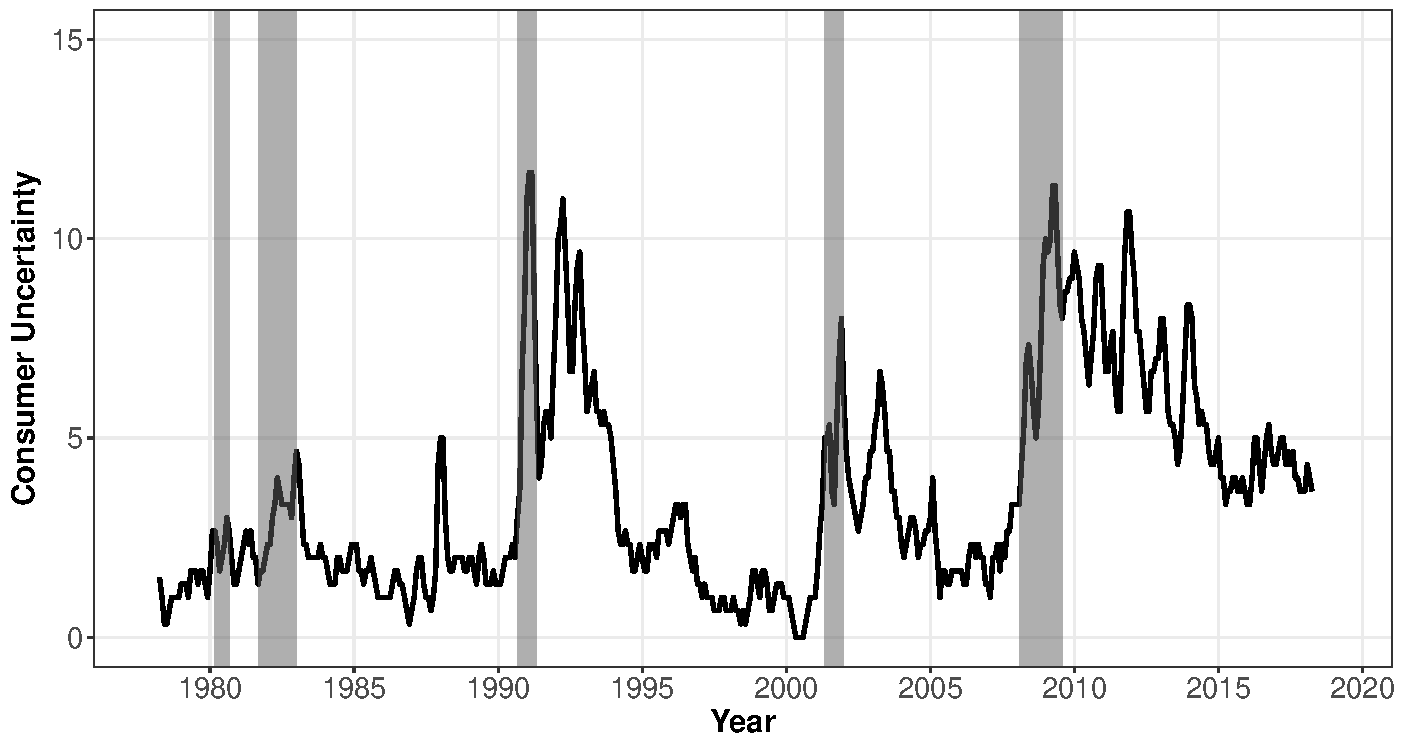
\includegraphics[trim=1cm -2.5cm 0.8cm -1cm, width=0.95\textwidth]{michigan_plot.pdf}}
      \caption[Thomson Reuters/University of Michigan Survey of Consumers, Consumer Uncertainty.]{Thomson Reuters/University of Michigan Survey of Consumers, Consumer Uncertainty.}   \label{fig:michigan_plot}
\end{figure}

\begingroup
    \fontsize{8pt}{12pt}\selectfont
    Note to self:
\begin{itemize}
	\item \citet{orlikandveldkamp:14} go on and write: ``Another commonly cited measure of uncertainty is business or consumer confidence. The confidence survey asks respondents whether their outlook on future business or employment conditions is 'positive', negative or neutral.' These questions are about the direction of future changes and not about any variance or uncertainty. They may be correlated with uncertainty because uncertainty is counter-cyclical.\\
	\item Basu und Bundick (2017) und Ledu and Lui (2016) verwenden als Unsicherheitsmaße einmal nur den VIX und einmal die ratio aus dem Michigan Survey (das ganze ist einfach direkt von der homepage herunterladbar)\\
	\item Here I should also refer to \citet{bachmannetal:13}.
	\item We should make use of the uncertainty measure used in \citet{bachmannetal:13} and also create a similar plot compared to their Figure 22. Although the data for the IFO index is only available as of 1980, we could still make use of this and, e.g., compare the volatility indicator that \citet{bloom:09} uses with the uncertainty indicator used by \citet{bachmannetal:13}. Interestingly, \citet{bachmannetal:13} even write in their footnote 16: ``We follow here Bloom's (209) timing convention for stock market volatility.''
	\item another approach is mentioned in \citet{bachmannetal:13} where they write on p. 27: `We also run an analogous SVAR with the 30 year corporate bond spread as the uncertainty measure. It is clear that negative long-run innovations have significant impact on uncertainty.''
\end{itemize}
\endgroup




\subsection{Economic Policy Uncertainty Index: \citet{bakeretal:15}}
\label{sec:epuindex}

\begingroup
    \fontsize{8pt}{12pt}\selectfont
    Note to self:
\begin{itemize}
	\item  BBD-index following \citet{bakeretal:15}\\
The IMF Working Paper (Measuring Global and Country-Specific Uncertainty) is a very helpful resource because: (1) They compare various uncertainty measures and also give a hint of from where to retrieve news-based uncertainty-measures!
	\item \citet[p. 1593]{bakeretal:16} write: ``We develop a new index of economic policy uncertainty (EPU) based on newspaper coverage frequency. Several types of evidence - including human readings of 12,000 newspaper articles - indicate that our index proxies for movements in policy-related economic uncertainty. Our U.S. index spikes near tight presidential elections, Gulf Wars I and II, the 9/11 attacks, the failure of Lehman Brothers, the 2011 debt ceiling dispute, and other major battles over fiscal policy.''
	\item \citet[p. 1593]{bakeretal:16} write: ``At the macro level, innovations in policy uncertainty foreshadow declines in investment, output, and employment in the United States and, in a panel vector autoregressive setting, for 12 major economies.''
	\item \citet[p. 1593]{bakeretal:16} write: ``Extending our U.S. index back to 1900, EPU rose dramatically in the 1930s (from late 1931) and has drifted upward since the 1960s.'' --> This is a sentence that we should include in our description of the time-series itself!
\end{itemize}
\endgroup


\begin{figure}[h]
   \centering
   \setlength\fboxsep{0pt}
   \setlength\fboxrule{0pt}
   \fbox{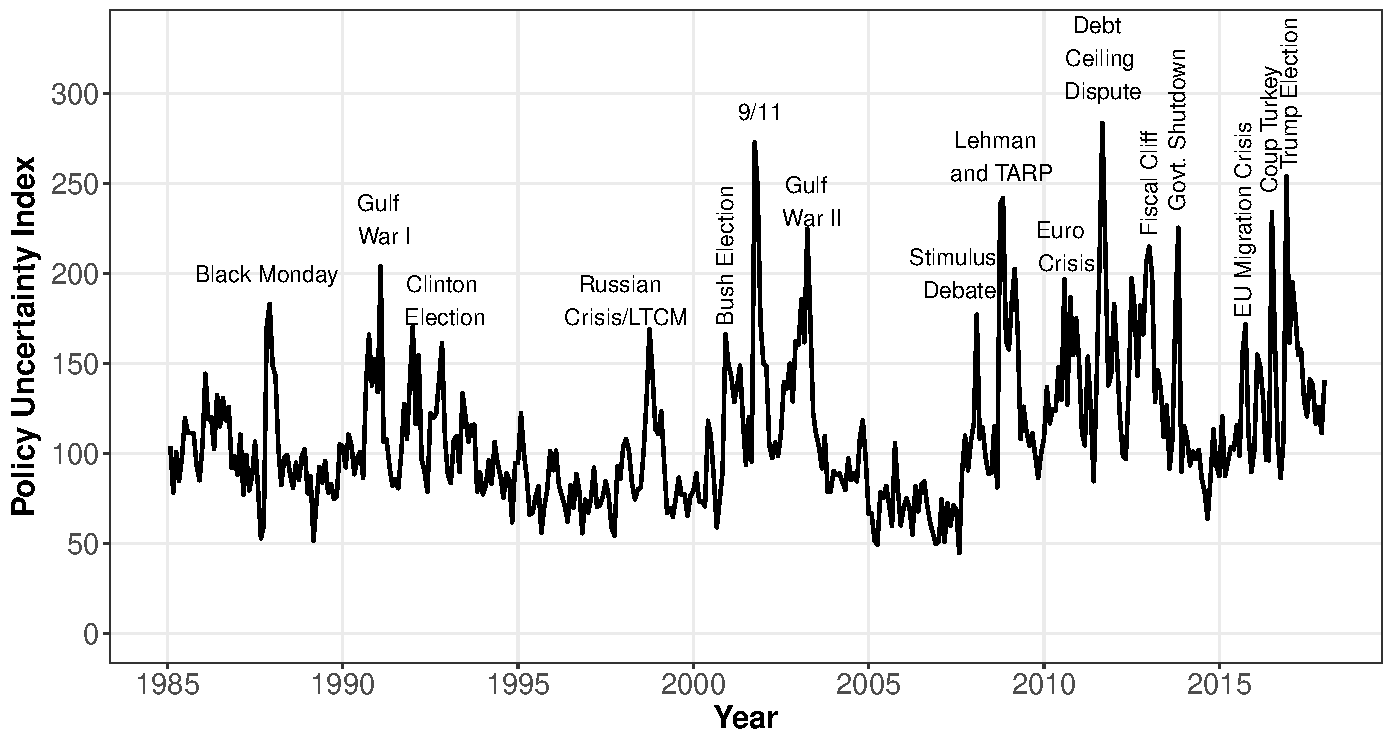
\includegraphics[trim=1cm -2.5cm 0.8cm -1cm, width=0.95\textwidth]{epu_index_plot.pdf}}
      \caption[EPU Index for the United States.]{EPU Index for the United States.
      \textit{Note:} Index reflects scaled monthly counts of articles containing 'uncertain' or 'uncertainty', 'economic' or 'economy, and one or more policy relevant terms: 'regulation', 'federal reserve', 'deficit', 'congress', 'legislation', or 'white house'. The series is normalized to mean 100 from 1985-2009 and based on queries run on 2 February, 2015 for the USA Today, Miami Herald, Chicago Tribune, Washington Post, LA Times, Boston Glove, SF Chronicle, Dallas Morning News, NW Times, and the Wall Street Journal.\\
      Original Figure Iå in \citet{bakeretal:15} spans until 2015. We have taken all available values until April 2018, inclusive.}   \label{fig:epuindex}
\end{figure}



\subsection{[Google Trends-based Index: \citet{bontempietal:16} and \citet{castelnuovoandtran:17}]}
\label{sec:googletrends}
\href{https://medium.com/google-news-lab/what-is-google-trends-data-and-what-does-it-mean-b48f07342ee8}{Google Trends is a freely available Google service derived from Google search data. As such it is a powerful tool when it comes to the exploration of global reactions to major events based on what people search for world-wide.}\footnote{For more information see \url{https://support.google.com/trends/?hl=en\#topic=6248052}.} The data that Google makes available thereby can be filtered in two ways: (i) \textbf{real time}, which is a random sample of searches from the last seven days and (ii) \textbf{non-real time} which is a random sample of the full Google dataset which can go back anywhere from 2004 to ca. 36 hours ago.\footnote{The algorithm reverts to sampling because otherwise the query to trillions of Google searches could not be executed within a reasonable amount of time.} 
\\
\\
The feature that actually makes Google Trends useful is that it is normalized, meaning that when looking at the search interest for a specific topic over time, the presented data points show \textit{the proportion of all searches on all topics on Google at that particular time and location}. Only this makes the search interest for a particular topic across time (and potentially additionally across locations) comparable in the first place. The reported numbers are indexed to 100 (with 100 standing for the maximum search interest for a particular time and location selected).

\begin{figure}[h]
   \centering
   \setlength\fboxsep{0pt}
   \setlength\fboxrule{0pt}
   \fbox{\includegraphics[trim=1cm -2.5cm 0.8cm -1cm, width=0.95\textwidth]{gtu_index_plot.pdf}}
      \caption[Google Trends Uncertainty (GTU) index.]{Google Trends Uncertainty (GTU) index.
      \textit{Note:} Sample: 2004M1-2016M12. Index constructed by weighting search queries related to a battery of country-specific keywords as explained above and normalized to have mean = 100 and standard deviation = 30.}   \label{fig:gtuindex}
\end{figure}

\citet[p. 3]{bontempietal:16} summarize the rationale to use Internet searches, stating that ``[h]igher levels of uncertainty are likely to result in a greater appetite for knowledge, and consequently in a more intense use of tools capable of gathering further information.'' Hence, the linkage between uncertainty about the outcome of a specific political or economic event and the potential resulting intensity of Internet searches which is assumed to mirror individuals' perceived uncertainty is exploited. \\
\\
\citet{castelnuovoandtran:17} construct Google Trends-based uncertainty indices (henceforth called GTU indices) for the United States and Australia.\footnote{In the following we will only consider the case of the US and therefore also continue to speak of only one GTU \textit{index}.} Their index is based on frequently mentioned keywords appearing in reference economic documents like the Federal Reserve's Beige Book\footnote{The Beige Book gathers anecdotal information on current economic conditions based on interview with, among others, key business contacts, economists and market experts. See \url{https://www.federalreserve.gov/monetarypolicy/beige-book-default.htm} for more information.} (for the United States) in connection to the word \textit{uncertainty}. The authors report to have subjectively selected relevant search-terms from various editions of the Beige Book resulting in 79 keywords for the U.S. (the complete list is available in the appendix of \citealp{castelnuovoandtran:17}). \\
\\
The aggregation based on the 79 identified keywords is then performed as follows (see \citet{castelnuovoandtran:17}): \\
As already indicated above, Google Trends data reports the frequency of a particular search term relative to the total search volume $S_{i, j, m, c}$ by dividing each raw data point $R_{i, j, m, c}$ (the frequency of a word $i$ in a group of searched words $j$ in period $m$ in location $c$) by the total searches $T$ in the same period/location so that $S_{i, j, m, c} = \frac{R_{i, j, m, c}}{T_{m, c}}$. 





\subsection{Macro Uncertainty Index: \citet{juradoetal:15}}
\label{sec:macrouncertainty}
Especially in contrast to stock market volatility and/or cross-sectional dispersion measures frequently deployed in uncertainty studies, \citet{juradoetal:15} have designed a computationally and data-intensive approach by making use of a rich set of time series, computing the conditional volatility of the unforecastable component of the future value of each of these series and finally aggregating these conditional volatilities into one composite index.\footnote{Note that, apart from practical issues, \citet[p. 1191]{juradoetal:15} themselves explain the reliance on (most likely revised) ``historical'' data (instead of ``real time'' data) with their goal of forming the ``[...] most historically accurate estimates of uncertainty at any given point in time in [their] sample''.}\\
\\
To set their approach apart from other commonly used uncertainty measures, \citet[p. 1178]{juradoetal:15} argue that ``[...] what matters for economic decision making is not whether particular economic indicators have become more or less variable or disperse \textit{per se}, but rather whether the economy has become more or less \textit{predictable}; that is, less ore more uncertain.''\\
\\
To formalize the rationale behind their approach, they define the $h$-period ahead uncertainty in the variable $y_{jt} \in Y_t = (y_{1t}, \ldots, y_{N_{y}t})'$, denoted by $U^t_{jt}(h)$, as the conditional volatility of the purely unforecastable component of the future value of the series, i.e.,
\begin{equation} \label{eq:juradoetal_1}
U^t_{jt}(h) \equiv \sqrt{\mathbb{E}\Big[(y_{jt+h} - \mathbb{E}[y_{jt+h}|I_t])^2|I_t\Big]},
\end{equation}
where the expectation $\mathbb{E}(\cdot|I_t)$ is taken with respect to information $I_t$ available to economic agents at time $t$. Hence, if the expectation today (conditional on all available information) of the squared error in forecasting $y_{jt+h}$ rises, uncertainty in the variable increases. The individual uncertainties at each date are then aggregated into a \textit{macroeconomic uncertainty} index by using aggregation weights $w_j$ as follows:
\begin{equation} \label{eq:juradoetal_2}
U^t_{jt}(h) \equiv plim_{N_{y}\to\infty} \sum_{j=1}^{N_y} w_j U_{jt}^y(h) \equiv \mathbb{E}_w \Big[U_{jt}^y(h)\Big]
\end{equation}

Based on the above definitions, \citet{juradoetal:15} emphasize two features that are central to their approach:
\begin{enumerate}
	\item they distinguish between \textit{uncertainty} in a series $y_{jt}$ and its \textit{conditional volatility} and argue that the proper measurement of uncertainty requires the removal of the entire forecastable component $\mathbb{E}[y_{jt+h}|I_t]$ before the computation of the conditional volatility; without accounting for this, the argument goes, forecastable variation is erroneously classified as ``uncertainty''. According to \citet{juradoetal:15}, this is taken into account only in very few occasions in the literature.
	\item they claim that macroeconomic uncertainty is ``a measure of the common variation in uncertainty across many series'' and not equal to the uncertainty in any single series $y_{jt}$; \citet{juradoetal:15} see this as an important argument because of uncertainty-based theories of the business cycle that typically require the existence of common (often countercyclical) variation in uncertainty across large numbers of series; \citet{juradoetal:15} hence put their econometric estimation of uncertainty insofar to test, as they expect to find evidence of such an aggregate uncertainty factor common to many series, if the above assumption turns out to be correct.
\end{enumerate}

\citet{juradoetal:15}'s econometric approach then consists of three parts:
\begin{enumerate}[i]
	\item estimation of the forecastable component $\mathbb{E}[y_{jt+h}|I_t]$: this is achieved by, first, running a factor analysis on a large set of predictors (132 macro time series) $\{X_{it}\}, i = 1, 2, \dots, N$ whose linear span/hull comes as close as possible to $I_t$; second, making use of the formed factors, $\mathbb{E}[y_{jt+h}|I_t]$ is then approximated by means of a diffusion index forecasting model ideal for data-rich environments (the diffusion indices can then be treated as known in the subsequent steps)
	\item with the definition of the $h$-step-ahead forecast error as $V_{jt+h}^y \equiv y_{jt+h} - \mathbb{E}[y_{jt+h}|I_t]$, \citet{juradoetal:15} estimate the conditional volatility of this forecast error, i.e., $\mathbb{E}[(V_{t+h}^y)^2|I_t]$ at time $t$ by specifying a parametric stochastic volatility model for both the one-step-ahead prediction errors in $y_{jt}$ and the analogous forecast errors for the factors (from step i above); \\
	these volatility estimates are then used to recursively compute the values of $\mathbb{E}[(V_{t+h}^y|I_t]$ for $h > 1$. 
	\item in the last step, the \textit{macroeconomic uncertainty} index $U_t^y(h)$ is constructed from the individual uncertainty measures $U_{jt}^y(h)$ where the base-case is the equally-weighted average of individual uncertainties
\end{enumerate}

While \citet{juradoetal:15} apply their approach to two large dataset with economic time-series (one monthly dataset containing hundreds of macroeconomic and financial indicators and one quarterly dataset containing 155 firm-level observations on profit growth normalized by sales), here we only confine ourselves to the former, i.e., their \textit{common macro uncertainty} index.

Their resulting estimated measure of time-varying uncertainty is plotted in Figure~\ref{fig:macroUncertainty_index} and reveals 'only' three big episodes of uncertainty: the months during the recessions from 1973-1974 and 1981-1982 and the months during the Great Recession of 2007-2009 (being the most striking episode of heightened uncertainty, followed by the 1981-1982 recession as a close second).\footnote{See Table~\ref{tab:macro_shocks} below for the exact dates including the maximum value for the index for each identified episode of high uncertainty.}\footnote{\citet{juradoetal:15} report that a closer look at the estimates reveals that the three series with the highest uncertainty are a producer price index for intermediate materials, a commodity spot price index, and employment in mining between 1973:11 and 1975:3, the Fed funds rate, employment in mining, and the three months commercial paper rate for the 1980:1 and 1982:11 episode and the monetary base, non-borrowed reserves and total reserves between 2007:12 and 2009:6. \citet{juradoetal:15} conclude these results to be consistent with the historical account.}

\begin{figure}[!ht]
   \centering
   \setlength\fboxsep{0pt}
   \setlength\fboxrule{0pt}
   \fbox{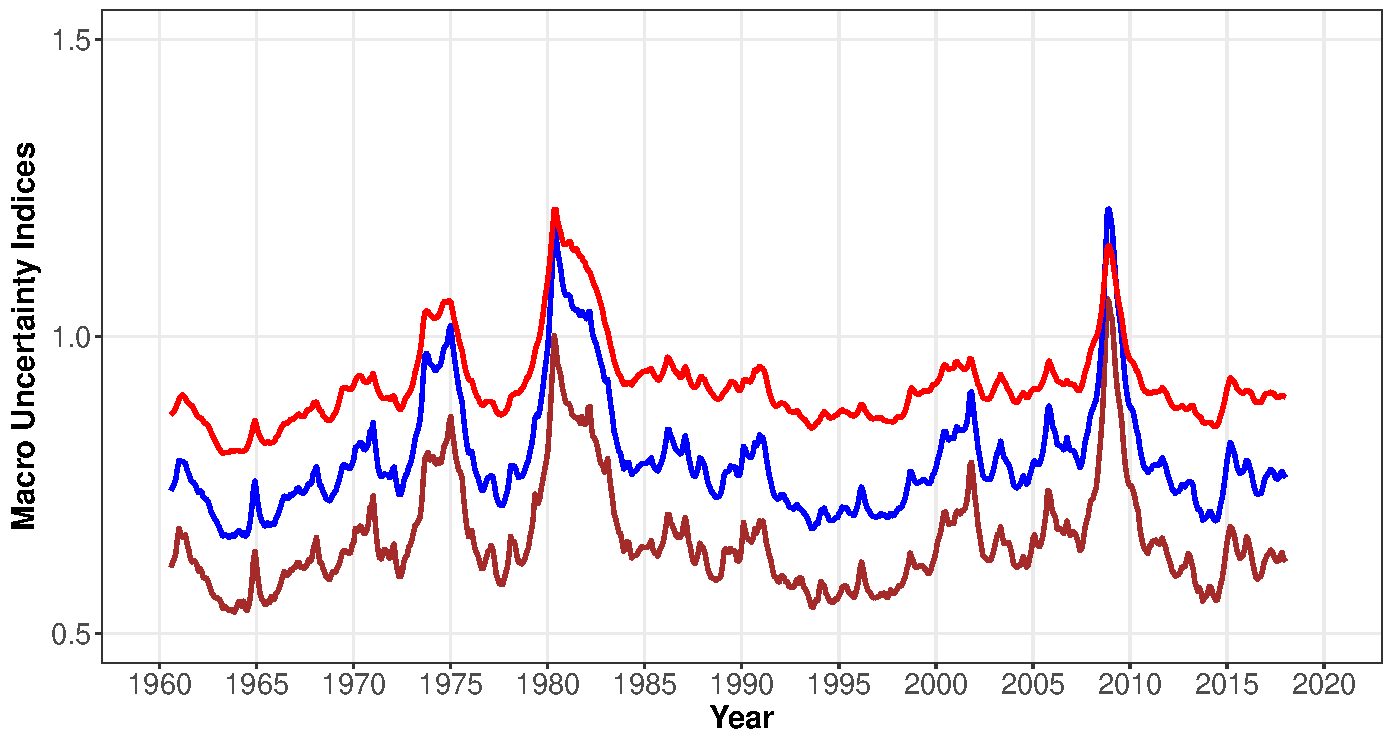
\includegraphics[trim=1cm -1.5cm 0.8cm -1cm, width=0.95\textwidth]{macroUncertainty_index_plot.pdf}}
      \caption[Aggregate Uncertainty: $h = 1, 3, 12$.]{Aggregate Uncertainty: $h = 1, 3, 12$.
      \textit{Note:} Horizontal lines indicate 1.65 standard deviations above the mean of each series. Data are monthly and span the period 1960:7-2017:12. Red shaded areas correspond to dates where volatility series exceeds 1.65 standard deviation above the mean of the h1-series. Grey shaded areas denote NBER recession dates in the US.\\
      Original Figure 1 in \citet{juradoetal:15} spans until 2011. We have taken all available values until December 2017, inclusive.}   \label{fig:macroUncertainty_index}
\end{figure}

\begin{table}[t]
\begin{center}
\caption{Periods of high uncertainty according to macro uncertainty index h=1.}
\scalebox{0.8}{
    \begin{tabular}{ccccc}
    \hline
         Start & End & Duration & Maximum Year/Month & Maximum Value \\ \hline
        Sep 1974 & Mar 1975 & 7 months & Jan 1975 & 0.87 \\
        Jan 1980 & Aug 1982 & 31 months & May 1980 & 1.00 \\
        Jul 2008 & Sep 2009 & 15 months & Nov 2008 & 1.06 \\
        \hline
        \hline
    \end{tabular}
}
\label{tab:macro_shocks}
\end{center}
\end{table}


The IMF Working Paper (Measuring Global and Country-Specific Uncertainty) is a very helpful resource because: (4) They also succinctly describe the uncertainty-measure developed by Jurado et al (which is very complicated!)




\subsection{Additional Parts for Later Usage}
\citet{orlikandveldkamp:14} discuss data used to proxy for uncertainty in Section 5 and offer a useful taxonomy which we could make use of as well! They write: ``Our model generates a measure of economic uncertainty. In this section, we describe the commonly used proxies of uncertainty, analyze their theoretical relationship with conditional variance and then compare their statical properties to those of our measure. \citet{orlikandveldkamp:14} mention the following uncertainty measures:\\
\\
\\
\\
\\
Another interesting sentence that is written in \citet{bachmannetal:13}, p. 10: ``Measuring the subjective uncertainty of decision makers is inherently difficult. Ideally, one would like to elicit a subjective probability distribution over future events from the managers, as has been done in Guiso and Parigi (1999) for Italian firms. with this probability distribution it is straightforward to compute a measure of subjective uncertainty for firms' decision makers. However, to the best of our knowledge such probability distributions are not available repeatedly and over long time horizons. Therefore, reserachers have to rely on proxies.'' \\
\\
\\
\\
Note to self: 
\begin{itemize}
	\item I could potentially at some point refer to economic sentiment indicators like \url{https://www.oenb.at/en/Statistics/Standardized-Tables/
	Economic-and-Industry-Indicators/Economic-Indicators/Economic-Sentiment-Indicator-for-the-Euro-Area.html} or \url{https://data.europa.eu/euodp/data/dataset/c04BuUz6WXIQGJkHPwLug}
\end{itemize}

\subsection{A Critique of the Various Measures}
\begin{itemize}
	\item Comparing the VXO to their own macro uncertainty index, \citet[p. 1201]{juradoetal:15} write that ``[...] it is difficult to imagine that the level of macro uncertainty in the economy in October 1987 (not even a recession year) was on par with the recent financial crisis.''
	\item \citet{orlikandveldkamp:14} go on and write: ``Other proxy variables for uncertainty are informative, but have a less clear connection to a conditional variance definition of uncertainty.' (then they go on and write about business or consumer confidence, market volatility index (VIX), etc.)'
	\item mentioned in \citet[p. 1182]{juradoetal:15}: ``[...] we emphasize here that the measures of dispersion and stock market volatility studied may or may not be tightly linked to true economic uncertainty. Indeed, one of the most popular proxies for uncertainty is closely related to financial market volatility as measured by the VIX, which has a large component that appears driven by factors associated with time-varying risk-aversion rather than economic uncertainty (see \citet{bekaertetal:13}) 
	\item similarly, \citet[p. 12]{bontempietal:16} write: ``The (i) VIX is used in many empirical studies (most prominently in \citet{bloom:09}). But one caveat that emerges from the use of the VIX to proxy uncertainty concerns its ability to represent macroeconomic uncertainty, since it is based on stock market information alone. According to \citet{bekaertetal:13}, the VIX does not only reflect uncertainty but can be broken down into uncertainty and risk-aversion. Since risk aversion accounts for a sizeable part of the VIX,\footnote{For this reason, the VIX is usually referred to as the ``fear index'' (see, e.g., \citet{whaley:00}).}, even more caution should be taken when considering it as a proxy of macro-economic uncertainty.
	\item in their non-technical summary, \citet{bekaertetal:13} write: ``Second, Bloom (2009) and Bloom, Floetotto and Jaimovich (2009) show that heightened
“economic uncertainty” decreases employment and output. It is therefore conceivable that the
monetary authority responds to uncertainty shocks, in order to affect economic outcomes.
However, the VIX index, used by Bloom (2009) to measure uncertainty, can be decomposed
into a component that reflects actual expected stock market volatility (uncertainty) and a
residual, the so-called variance premium, that reflects risk aversion and other non-linear pricing
effects, perhaps even Knightian uncertainty. Establishing which component drives the strong
co-movements between the monetary policy stance and the VIX is therefore particularly
important''
	\item related to our empirical analysis: \citet[p. 1184]{juradoetal:15} write: ``An important unresolved issue for empirical analysis of uncertainty concerns the persistence of uncertainty shocks. [...] Researchers (e.g., Schaal 2011) have argued that empirical proxies for uncertainty, such as the cross-sectional dispersion in firms' sales growth, are not persistent enough to explain the prolonged levels of unemployment that have occurred during and after some recessions, notably the 2007-2009 reession and its aftermath. Here we provide new measures of uncertainty and its persistence, finding that they are considerably more persistent than popular proxies such as stock market volatility and measures of dispersion.
	\item With regard to cross-sectional dispersion measures in $N_A$ analysts' or forms' subjective expectations as a measure of uncertainty, \citet[p. 1182]{juradoetal:15} also have a very strong opinion: ``A separate strand of the literature focuses on cross-sectional dispersion in $N_A$ analysts' or firms' subjective expectations as a measure of uncertainty:
	\begin{equation}\label{eq:juradoetal_3}
D^A_{jt}(h)  = \sqrt{\sum_{k=1}^{N_{A_t}} w_k^A \Big(y_{jt+h} - \mathbb{E} (y_{jt+h}|I_{{A_k}, t})\Big)^2},
	\end{equation}
	where $I_{{A_k}, t}$ is the information of agent $k$ at time $t$, and $w_k^A$ is the weight applied to agent $k$. One potential advantage of using $D^A_{jt}(h)$ as a proxy for uncertainty is that is treats the conditional forecast of $y_{jt+h}$ as an observable variable, and therefore does not require an estimation of $\mathbb{E} (y_{jt+h}|I_{{A_k}, t})$. \citet{bachmannetal:13} follow this approach using a survey of German firms and argue that uncertainty appears to be more an outcome of recessions than a cause, contrary to the predictions of theoretical models such as \citet{bloom:09} and others. [...] While analysts' forecasts are interesting in their own right, there are several known drawbacks in using them to measure uncertainty. First, subjective expectations are only available for a limited number of series. For example, of the 132 monthly macroeconomic series we will consider in this paper, not even one-fifth have corresponding expectations series. Second, it si not clear that the responses elicited from these surveys accurately capture the conditional expectations of the economy as a whole. The respondents typically sampled are practitioner forecasters; some analysts' forecasts are known to display systematic biases and omit relevant forecasting information (So, 2013), and analysts may have pecuniary incentives to bias their forecasts in a way that economic agents would not. Third, disagreement in survey forecasts could be more reflective of differences in opinion than of uncertainty. Fourth, Lahiri and Shen (2010) show that, even if forecasters are unbiased, disagreement in analysts' point forecasts does not equal (average across analysts) forecast error uncertainty unless the variance of accumulated aggregate shocks over the forecast horizon is zero. \citet{bachmannetal:13} acknowledge these problems and are careful to address them by using additional proxies for uncertainty, such as an ex post measure of forecast error variance based on the survey expectations. \\
	
	
	
	\item Further, \citet{juradoetal:15} (pp. 1178) argue, that ``unfortunately, the conditions under which common proxies are likely to be tightly linked to the typical theoretical notion of uncertainty may be quite special. For example, stock market volatility can change over time even if there is no change in uncertainty about economic fundamentals, if leverage changes, or if movements in risk aversion or sentiment are important drivers of asset market fluctuations.\\
Cross-sectional dispersion in individual stock returns can fluctuate without any change in uncertainty if there is heterogeneity in the loadings on common risk factors. similarly, cross-sectional dispersion in firm-level profits, sales, and productivity can fluctuate over the business cycle merely because there is heterogeneity in the cyclicality of firms' business activity.'' 
	\item \citet[p. 13]{bontempietal:16} write: ``Although independent of any single observable economic indicator or event, the macroeconomic uncertainty measure following \citet{juradoetal:15} is a computationally intensive black box that is not directly linked to the uncertainty perceived by the general public.  
\end{itemize}

\section{Comparison of Selected Measures}
\begin{figure}[!ht]
   \centering
   \setlength\fboxsep{0pt}
   \setlength\fboxrule{0pt}
   \fbox{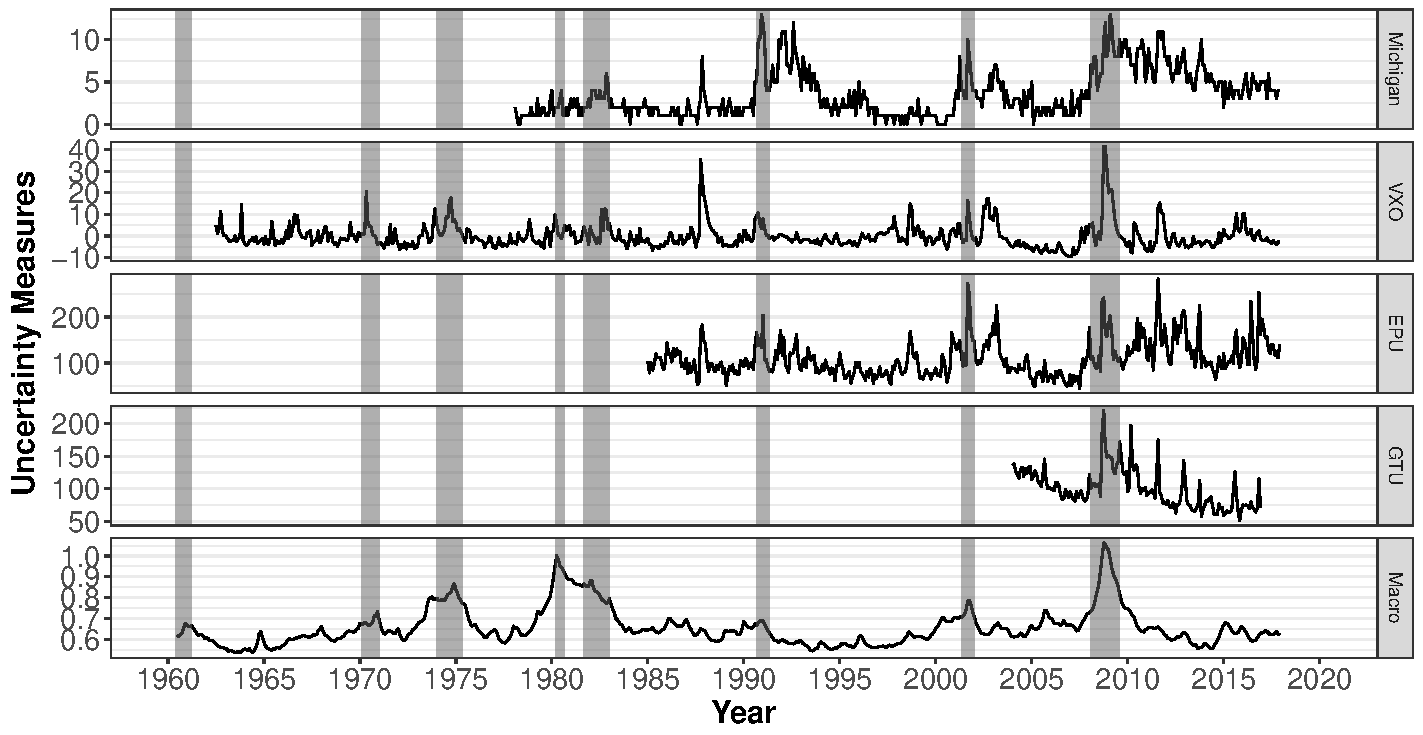
\includegraphics[trim=1cm -1.5cm 0.8cm -1cm, width=0.95\textwidth]{comparison_plot.pdf}}
      \caption[Comparison of uncertainty measures (facetted).]{Comparison of uncertainty measures (facetted).
      \textit{Note:} Shaded areas denote NBER recession dates in the US. Data frequencies are monthly. The macro uncertainty series starts in July 1960, the GTU in January 2004, the EPU in January 1985, the consumer uncertainty series (Michigan Survey) in February 1978 and the VXO/stock-market volatility series in July 1962.\\
      Note to self: We define high uncertainty events as months when either uncertainty measure was one standard deviation above its time series average. (still have to add these values to the plots!))}   \label{fig:comparison_plot}
\end{figure}


Figures \ref{fig:comparison_plot} (on different scales) and \ref{fig:comparison_plot_combined} (normalized to the same scale) show all uncertainty measures we have considered so far including NBER recessions for the U.S. A first preliminary visual inspection shows that similar to \citet{bachmannetal:13}'s assessment in their own comparison, almost all recession periods correspond to elevated uncertainty across all measures. Apart from this commonality, the VXO and EPU show much noisier fluctuations than e.g., the macro uncertainty index. And while the VXO and EPU show a similar trajectory prior to the crisis, the EPU remains elevated during most of the recovery period showing more variation including several spikes (comparable to the GTU over that period). At a first glance, this suggests that the EPU indeed reacts much stronger to the political turmoil in the past decade than financial markets themselves. \\
\\
The macro uncertainty index overall stands out with an overall smoother trajectory and marked spikes that correspond to recessions but also, as aptly formulated by \citet{juradoetal:15} themselves, significant independent variation as compared to the other commonly used uncertainty measures suggesting that ``[...] quantitatively important uncertainty episodes occur far more \textit{in}frequently\footnote{Italics added.} than what is indicated from common uncertainty proxies, but that when they \textit{do} occur, they display larger and more persistent correlations with real activity'' \citep[p. 1181]{juradoetal:15}. This observation can be confirmed by looking at Figures \ref{fig:comparison_plot} and \ref{fig:comparison_plot_combined} where increases in the macro uncertainty estimates are mostly associated with protracted recessions whereas more modest recessions are accompanied with smaller spikes. A period where the macro uncertainty index stands out is the recessionary period from 1980-1982: throughout this episode the index is highly elevated while other measures are comparatively low. The VXO on the other hand also shows spikes outside of recession periods that correspond to events exclusively related to stock-markets. For example, the large spike commonly on 'Black Monday' (October, 19th 1987) when stock markets experienced their largest single-day percentage decline ever recorded, is only visible in the MSoC (with a timely delay - almost not visible) and the EPU. The macro uncertainty index, however, barely moves around that time. Interestingly, the EPU shows the largest spike surrounding the years 2001-2001 (the dot-com bubble). 

\begin{landscape}
\begin{figure}[!t]
   \centering
   \setlength\fboxsep{0pt}
   \setlength\fboxrule{0pt}
   \fbox{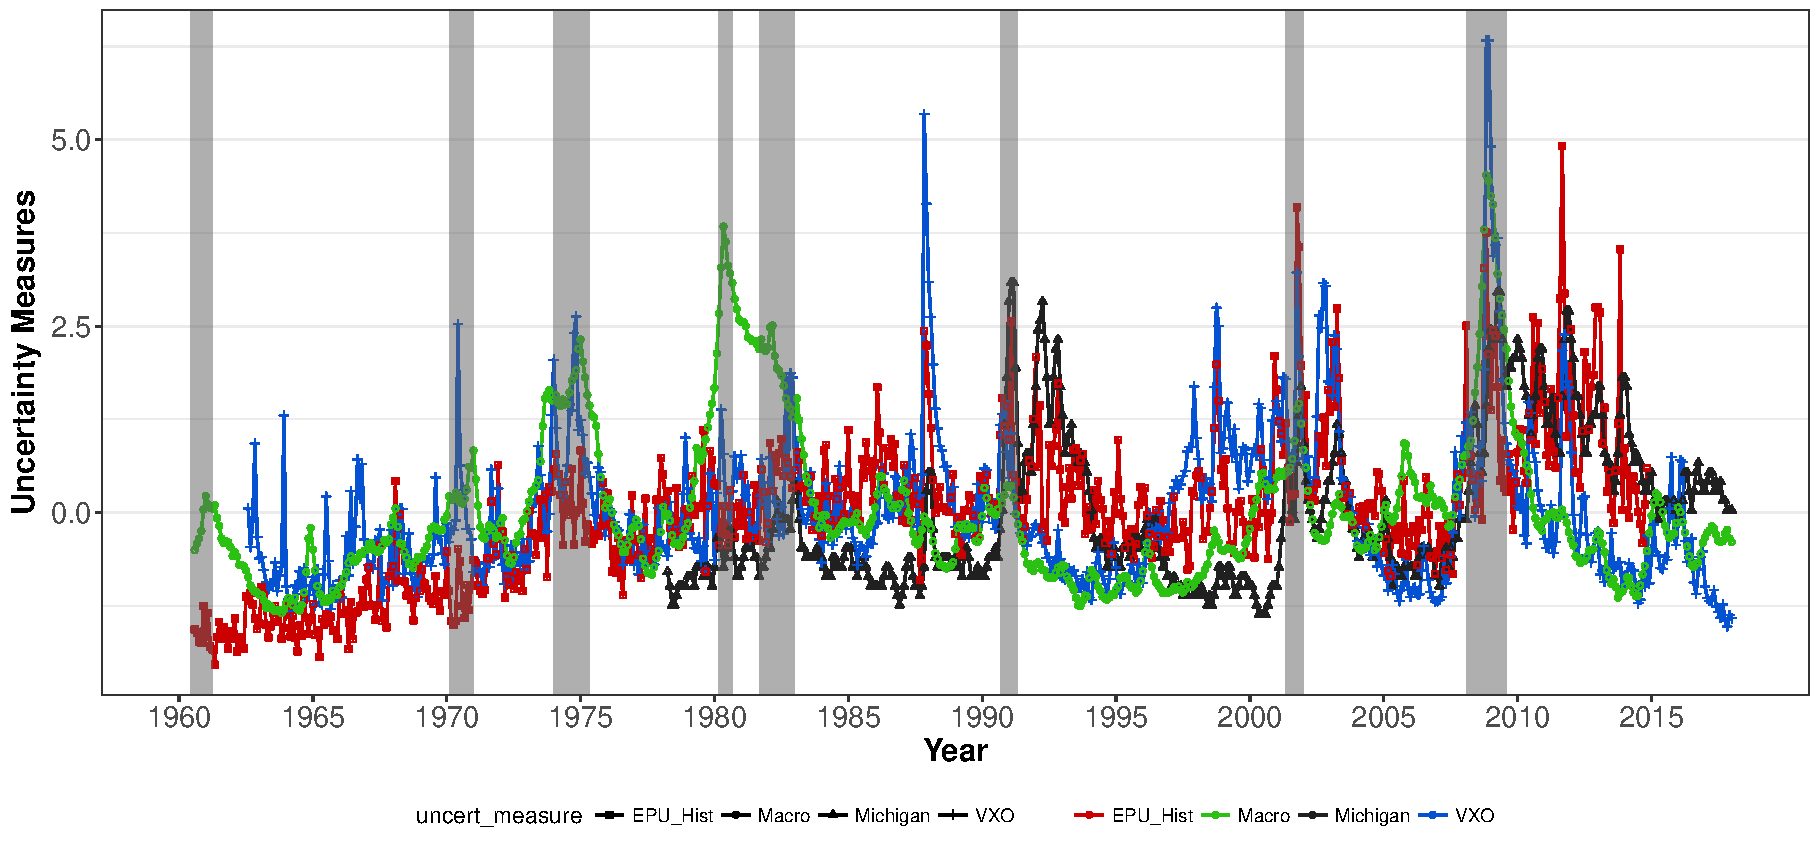
\includegraphics[trim=1cm -0.8cm 0.8cm 0.2cm, width=1.5\textwidth]{comparison_plot_combined.pdf}}
      \caption[Comparison of uncertainty measures (combined).]{Comparison of uncertainty measures (facetted).
      \textit{Note:} Shaded areas denote NBER recession dates in the US. Data frequencies are monthly. The macro uncertainty series starts in July 1960, the GTU in January 2004, the EPU in January 1985, the consumer uncertainty series in January 1978  and the VXO in July 1962.}   \label{fig:comparison_plot_combined}
\end{figure}
\end{landscape}

And while there is an overall comovement between the series, the identified episodes of substantial variation in the processes' dynamics suggest that ``[t]hese [time series] are clearly not measures of the same [latent] stochastic process [...]'' \citep[p. ]{orlikandveldkamp:14}.\\
\\
To prove the above statement, we will study the time-series properties of the various uncertainty measures in turn (results will be plotted below!).



\begin{table}[t]
\begin{center}
\caption{Correlation matrix of uncertainty measures.}
\scalebox{1}{ 
  \label{} 
	\begin{tabular}{@{\extracolsep{5pt}} cccccc} 
	\\[-1.8ex]\hline 
	\hline \\[-1.8ex] 
 	& MSoC & VXO & EPU & GTU & Macro \\ 
	\hline \\[-1.8ex] 
	MSoC & $1$ & $0.510$ & $0.600$ & $0.240$ & $0.340$ \\ 
	VXO & $0.510$ & $1$ & $0.530$ & $0.360$ & $0.630$ \\ 
	EPU & $0.600$ & $0.530$ & $1$ & $0.250$ & $0.150$ \\ 
	GTU & $0.240$ & $0.360$ & $0.250$ & $1$ & $0.620$ \\ 
	Macro & $0.340$ & $0.630$ & $0.150$ & $0.620$ & $1$ \\ 
	\hline \\[-1.8ex] 
	\end{tabular} 
}
\label{tab:correlations}
\end{center}
\end{table}


\begingroup
    \fontsize{8pt}{12pt}\selectfont
    Note to self:
\begin{itemize}
	\item here we should compare the statistical features at both the univariate (persistence, seasonality and variability over time) and multivariate (Granger causality and contemporaneous correlation) levels!! (compare to \citet{bontempietal:16})!!!! i.e., add time-series analysis of the uncertainty-measures! (like the one performed in Bontempi et al, 2015) to this section!
	\item add a table with the cross-correlation between the various measures!
	\item \citet{juradoetal:15} provide a table with summary statistics of their uncertainty measures for $h=1$. Their table reports the first-order autocorrelation coefficient, estimates of the half-life of an aggregate uncertainty innovation from a univariate autoregression (AR) for U_t(1), estimates of skewness, and kurtosis, and IP-Corr(k) is the (absolute) cross-correlation of Ut with industrial production growth at different leads and lags, k. The same statistics are reported for other uncertainty proxies,. Several statistical facts about their own estimate of aggregate uncertainty stands out in Table 1. \\
	Of course, these unconditional correlations are uninformative about the causal relation between uncertainty and real activity. All that can be said is that there is a strong coherence between uncertainty and real activity.
	\item Similar to \citet{juradoetal:15} I should add a table with summary statistics of the various volatility series (including their half-life, etc.)
	\item The following sentence is taken from \citet{bloom:09} where Bloom explains the rationale for taking the stock-market volatility: Here I should mention what is written in Bloom (2009): 'The evidence presented in Table I shows that a number of cross-sectional measures of uncertainty are highly correlated with time series stock-market volatility. Stock-market volatility has also been previously used as a proxy for uncertainty at the firm level (e.g., Leahy and Whited (1996) and Bloom, Bond, and Van REenen (2007)).'
	\item \citet[p. 1180]{juradoetal:15} write: ``Moreover, our estimate of macroeconomic uncertainty is far more persistent than stock market volatility: the response of macro uncertainty to its own innovation from an autoregression has a half-life of 53 months; the comparable figure for stock market volatility if four months.
	\item \citet[p. 3]{bontempietal:16} write: ``The three previous approaches al have their pros and cons. On the one hand, the pre-selection of directly obesrvable specific events is easy to perceive but somewhat arbitrary. On the other hand, the methodological approaches that extract uncertainty estimates from latent processes are statistically and economically sound but are also very complex black boxes not strictly related to observable indicators of uncertainty.''
	\item the differences between the macro uncertainty index of \citet{juradoetal:15} and other uncertainty measures cause \citet[p. 1180]{juradoetal:15} to conclude: ``Taken together, the findings imply that most movements in common uncertainty proxies, such as stock market volatility (the most common), and measures of cross-sectional dispersion, are not associated with a broad-based movement in economic uncertainty as defined in (2). This is important because it suggests that much of the variation in common uncertainty proxies is not driven by uncertainty.
\end{itemize}
\endgroup



\section{Some Stylized Facts}
Here I should replicate some of the stylized facts that Bloom has mentioned in his 2012 paper as well as in the corresponding Power-Point-Presentation!\\
\\
I have to read the review article from Nicholas Bloom where he starts the abstract with: ``This review article tries to answer four questions: (i) what are the stylized facts about uncertainty over time; (ii) why does uncertainty vary; (iii) do fluctuations in uncertainty matter; and (iv) did higher uncertainty worsen the Great Recession?



%%%%%%%%%%%%%%%%%%%%%%%%%%%%%%%%%%%%%%%%%%%%%%%%%%%%%%%%%%
%%%%%%%%%%%%%%%%%%%%%%%%%%%%%%%%%%%%%%%%%%%%%%%%%%%%%%%%%%
%%%%%%%%%%%%%%%%%%%%%%%%%%%%%%%%%%%%%%%%%%%%%%%%%%%%%%%%%%
\chapter{Related Literature}
\label{UncertaintyandBusinessCyclesRelatedLiterature}
The literature that investigates the linkages of uncertainty on various macroeconomic aggregates (and beyond) is extensive including both empirical and theoretical work. An often-cited theoretical study which is seen as a pioneering work in the field of uncertainty-studies is \citet{bernanke:83} who investigates optimal investment decisions under uncertainty in an oil cartel and finds that high uncertainty causes firms to postpone investments and hiring in an environment where investment projects cannot easily be undone and labor market laws cause changes to the labor force (either hires or fires) to be costly. Subsequent selected works include, for example, \citet{rameyandramey:95}, \citet{aghionetal:05}, \citet{mills:00} and \citet{imbs:07} on the relationship of volatility and growth, \citet{leahyandwhited:96} and \citet{bloometal:07} on the effect of uncertainty on investment, \citet{barlevy:04} and \citet{gilchristandwilliams:05} on the effects of uncertainty on business cycles, etc.\footnote{Note that the list of studies is not supposed to be exhaustive.} \\
\\
The growing body literature that has recently started to systematically study economic uncertainty in an attempt to understand its origins and the \textit{potential} causal effects of time-varying economic uncertainty on macroeconomic fluctuations (business cycles) largely has one thing in common: in a VAR context, uncertainty shocks seem to have a negative effect on output (or proxies thereof such as industrial production or employment). But as summarized by \citet[p. 23]{bontempietal:16}, ``[...] this key finding is only robust in regard to the uncertainty impact in the short run, whereas in the long run different works have pointed to somewhat heterogeneous output responses.'' \\
\\
The study whose results serve as a benchmark for our own analysis by replicating parts of it in Section~\ref{sec:EmpiricalAnalysis} below is \citet{bloom:09} who proposed uncertainty shocks as a 'new' driver of business cycles and triggered much of the literature in subsequent years. \citet{bloom:09} himself links his work with earlier publications of \citet{bernanke:83} and \citet{hassler:96} and conducts a comprehensive analysis of the impact of uncertainty shocks on business cycle fluctuations by (1) building a model with a time-varying second moment from which he then simulates a macro uncertainty shock and (2) compares the results to the impulse response functions of vector autoregression (VAR) estimations on actual data. While the bulk of his work concentrates on the former, interestingly it is the latter (the empirical analysis using VARs) that has triggered much of the controversy in the literature. In particular, using 17 identified exogenous shocks, \citet{bloom:09} estimates VARs showing that volatility shocks generate a short-run drop in industrial production of 1\% which last for about 6 months and subsequently creates a longer-run overshoot. In his setting, these results are robust to the effect of an uncertainty shock on employment and a range of alternative approaches (including variable ordering, variable inclusion, shock definitions, shock timing, and detrending).\\
\\
Contrary to Bloom's findings when using stock market volatility as a proxy for uncertainty, \citet{juradoetal:15} and \citet{bachmannetal:13} using forecast-based measures find a rather different response-pattern: their VARs show a sharp reduction in output at impact whose effect is far more persistent lasting for a couple of years after the shock with no signs of the overshooting effect as in \citealp{bloom:09}).\\
\\
While \citet{bloom:09} sees a confirmation for the 'wait-and-see approach' (Maybe I should add here a sentence starting with 'Central to Bloom's argumentation is the 'wait-and-see approach' and then explain the intuition behind it as outlined in \citet{bachmannetal:13}) according to his results, whereas \citet{bachmannetal:13}, using survey data get contrary predictions: 
\\
citet{bachmannetal:13} write on p. 28: ``This is at least suggestive evidence that uncertainty is a concomitant factor of bad economic times rather than a causal factor for them.''

Here I then should summarize the papers that refer to Bloom's paper and everything related to papers that study the effect of uncertainty on business cycles.
Here I should mention that uncertainty is an ubiqitous concern of policymakers (and quote a few examples that also Bloom refers to both in Bloom (2009) and his presentation slides that are based on Bloom (2012)).\\
\\
Auch, wenn wir dann die Literatur zusammenfassen: alles richtig einbetten in meine Auseinandersetzung. Nicht einfach nur beschreiben, was in den Papern drinnensteht, sondern wie das related zu dem was ich bringe. Jeder Absatz der drinnensteht, muss einen Grund haben, warum er drinnensteht im Hinblick auf die Fragestellung usw. 

Also: wohldefinierte Fragestellung, überschaubare Methode, Resultate. Das sollten die Kernkompetenzen sein (dass alles sauber beschrieben ist und zugänglich abgebildet ist, dass man weiß woher die Daten kommen und alles replizierbar ist).
\\
\\
\citet{juradoetal:15} write on p. 1182: ``Bloom's VAR estimates suggest that uncertainty has an impact on output and employment in the six months after an innovation in these measures, with a rise in volatility at first depressing real activity and then increasing it, leading to an over-shoot of its long-run level, consistent with the predictions of models with uncertainty as a driving force of macroeconomic fluctuations. Bloom et al. (2012) also documented a relation between real activity and uncertainty as proxied by dispersion in firm-level earnings, industry-level earnings, total factor productivity, and the predictions of forecasters. A recurring feature of these studies is that the uncertainty proxies are strongly countercyclical.''
\\
\\
\citet{orlikandveldkamp:14} write

As formulated by \citet[p. 24]{bontempietal:16}, the results found in the literature to date raise the following questions:
\begin{enumerate}
	\item are uncertainty shocks temporary or permanent?
	\item is the degree of persistence of identified negative uncertainty effects related to the econometric specification and/or the particular uncertainty measure used?
	\item does the time span over which a model is estimated play any role?
\end{enumerate}

We want to discuss these questions in our penultimate Section~\ref{sec:EmpiricalAnalysis} below.

\chapter{Empirical Analysis}
\label{sec:EmpiricalAnalysis}
\begingroup
    \fontsize{8pt}{12pt}\selectfont
    Note to self:
\begin{itemize}
	\item  In line with the mainstream perspective and for the purpose of this work, we will elaborate below whether or not we can reasonably argue that the measures of uncertainty that we look at can indeed be regarded as exogenous sources of shocks within our empirical model. 
	\item Here in the introduction to the Empirical Analysis I should outline the intuition behind the benchmark-model that we are analyzing (\citet{bloom:09}) which \citet{bachmannetal:13} describe very well in their introduction to Section 2: ``Time-varying uncertainty at the firm level may have economic consequences when there is a degree of irreversibility to firm actions. For a concrete example, suppose that a firm faces fixed costs to adjusting the size of its labor force and/or physical capital stock. Suppose further that there is a mean-preserving spread on the distribution of future demand for the firm's product. With fixed adjustments costs, higher uncertainty over future demand makes new hiring and investment less attractive. The reason for this is intuitive - if a large fixed cost must be paid do adjust the firm'S labor or capital, then there is reason to minimize the number of times this cost must be paid. If the future is very uncertain (in the sense that demand could be either very high or very low relative to the present), then it makes sense to wait until the uncertainty is resolved to undertake new hiring and investment.'' --> ``An increase in uncertainty thus makes inaction relatively more attractive.'' 
\end{itemize}
\endgroup

We now want to devote the rest of this thesis to the study of the dynamic relationships between and responses of a set of key macroeconomic variables to innovations (we'll call them 'shocks' in the following) of the various uncertainty measures which we have introduced in Section~\ref{MeasuringUncertaintyandaHistoricalView}. Various models have been suggested/studied in the literature each of them suggesting a slightly different set of variables to include and/or ordering with which the variables enter the VAR. For us, the benchmark model with which we will start is \citet{bloom:09} (see Section~\ref{sec:VAR8}), followed by a macro VAR in the style of \citet{christianoetal:05} 

%\newpage
\section{The Benchmark Model: VAR-8 following \citet{bloom:09}}
\label{sec:VAR8}
The starting point of our estimations are VARs that \citet{bloom:09} used in his original contribution. The ordering as depicted in vector~\ref{eq:VAR8} below according to \citet[p. 630]{bloom:09} is based on the assumptions that shocks instantaneously influence the stock market (levels and volatility), then moves on to prices (wages, the consumer price index (CPI), and interest rates), and finally eventually affects quantities (hours, employment and output). In particular, \citet{bloom:09}'s rationale for including the stock-market levels as the first variable in the ordering is to ensure that the impact of stock-market levels is already controlled for when looking at the impact of volatility shocks. Further, \citet{bloom:09} detrends all variables that enter the VARs using the HP-filter (\citealp{hodrickandprescott:97}) apart from the uncertainty measure(s).\footnote{In vector~\ref{eq:VAR8} all variables that enter the VAR detrended are marked with a $c$-prefix to indicate that the variable denotes the remaining cycle-component after removal of the trend.}\\
\\
\citet{juradoetal:15} replicate \citet{bloom:09}'s VARs in their contribution, renounce to detrend the variables however, arguing that the HP filter uses information over the entire sample which makes it difficult to interpret the timing of an observation and report results using \citet{bloom:09}'s original detrended variables in their Appendix. 

\begin{equation} \label{eq:VAR8}
\text{VAR-8:} \begin{bmatrix} \text{c-log(S\&P500 Index)} \\ 
				      \text{uncertainty}\\ 
				      \text{c-federal funds rate}\\
				      \text{c-log(wages)}\\
				      \text{c-log(CPI)}\\
				      \text{c-hours}\\
				      \text{c-log(employment)}\\
				      \text{c-log(industrial production)}
	      \end{bmatrix}\text{,}
	      \begin{bmatrix} \text{log(S\&P500 Index)} \\ 
				      \text{uncertainty}\\ 
				      \text{federal funds rate}\\
				      \text{log(wages)}\\
				      \text{log(CPI)}\\
				      \text{hours}\\
				      \text{log(employment)}\\
				      \text{log(industrial production)}
	      \end{bmatrix}
\end{equation}

In Figure~\ref{fig:VAR8_HP_until2008} below we have plotted the (orthogonalized) impulse response functions (IRFs) to orthogonal shocks created from a Cholesky decomposition for the VAR-8 setting according to \citet{bloom:09}'s original contribution (i.e., all variables apart from the uncertainty measures detrended). While \citet{bloom:09} solely considers the VXO/volatility-series (and derived shock-measures in various flavors - one of which, the month with the maximum volatility in a series of months with extraordinarily high volatility, we call 'Bloom-Shock' here) as his uncertainty measure with its effect on industrial production (as a proxy for output) and employment, in the spirit of \citet{juradoetal:15} and \citet{bontempietal:16} we here report a full bank of IRFs for the selection of popularized uncertainty measures we have discussed in Section~\ref{sec:MeasuringUncertainty}: the original 'Bloom-shock' and the VXO/volatility-series (as used by \citealp{bloom:09}), the MSoC (as used by \citealp{leducandliu:16}), the EPU (as used by \citealp{bakeretal:15}), the GTU (as used by \citealp{bontempietal:16} and \citealp{castelnuovoandtran:17}) and finally the macro uncertainty index as introduced by \citet{juradoetal:15}.


\begin{figure}[!h]
   \centering
   \setlength\fboxsep{0pt}
   \setlength\fboxrule{0pt}
   \fbox{\includegraphics[trim=0cm 1.5cm -0.5cm 3cm, width=1\textwidth]{var8_plot_all_HP_until2008.pdf}}
      \caption[Impulse Response Functions of Production and Employment from Estimations of VAR-8 following \citet{bloom:09} using all uncertainty measures.]{Impulse Response Functions of Production and Employment from Estimations of VAR-8 following \citet{bloom:09} using all uncertainty measures. Variables enter the VAR-8 according to \ref{eq:VAR8}.\\
      \textit{Note:} Dashed lines show 68\% standard error bands. The data are monthly and span the period 1962:07-2008:06 for the Bloom-Shock and VXO/volatility series, 1978:02-2008:06 for the MSoC uncertainty series, 1975:01-2008:06 for the EPU and 1962:07-2008:06 for the Macro Uncertainty Index (both $h=1$ and $h=12$).}   \label{fig:VAR8_HP_until2008}
\end{figure}

\begin{figure}[!h]
   \centering
   \setlength\fboxsep{0pt}
   \setlength\fboxrule{0pt}
   \fbox{\includegraphics[trim=0cm 0.5cm -0.5cm 2.2cm, width=1\textwidth]{var8_plot_all_NoHP_until2008.pdf}}
      \caption[Impulse Response Functions of Production and Employment from Estimations of a modified version of the VAR-8 following \citet{bloom:09} using all uncertainty measures.]{Impulse Response Functions of Production and Employment from Estimations of a modified version of the VAR-8 \citet{bloom:09} using all uncertainty measures. Variables enter the VAR-8 according to \ref{eq:VAR8}.\\
       \textit{Note:} Dashed lines show 68\% standard error bands. The data are monthly and span the period 1962:07-2008:06 for the Bloom-Shock and VXO/volatility series, 1978:02-2008:06 for the MSoC uncertainty series, 1975:01-2008:06 for the EPU and 1962:07-2008:06 for the Macro Uncertainty Index (both $h=1$ and $h=12$).}   \label{fig:VAR8_NoHP_until2008}
\end{figure}

have to write into the caption that the length of the availability of the uncertainty measure is the limiting factors in all VARs (so for the macro uncertainty index, accordingly all data runs from 1960 until 2018, for the EPU from 1985 until 2018, for the GTU from 2004 to 2018 etc., etc.!!!)



A good sentence: 'The effect on impact, in contrast, is small.' 
Ein Satz aus Bachmann, den ich für meine eigene Arbeit verwenden sollte: "The next sectino discusses the wait-and-see mechanism and delivers a benchmark against which we compare our empirical results." (p. 4) --> Then I can replicate the results from Bloom and then show the results that local projections would produce.\\
\\
Note to self: \citet{bachmannetal:13} write on p. 5: ``In this section we give a brief overview of the ``wait-and-see'' mechanism that might give rise to uncertainty-driven fluctuations. In addition to providing a benchmark against which we can compare our empirical results, this exercise will also serve to motivate the use of high-frequency, sectoral data in examining the impact of uncertainty on economic activity.''\\
Another sentence that \citet{bachmannetal:13} use on p. 6: ``Figure 2 provides an example of an impulse response of output to an increase in uncertainty, replicated from the model in \citet{bloom:09}.


\section{Alternative Estimations I: VAR-11 following \citet{christianoetal:05}}
\label{sec:VAR11}
As mentioned by \citet{juradoetal:15} in their own estimations, \citet{christianoetal:05}'s studied VAR has the advantage of consisting of a set of variables whose dynamic relationships have been well studied/established in the literature. But because in their original contribution, \citet{christianoetal:05} use quarterly data, \citet{juradoetal:15} apply a slightly modified version of \citet{christianoetal:05}'s VAR to cover roughly the same sources of variation in the economy. This results in an 11-variable VAR whose ordering mimics the original model of \citet{christianoetal:05} as depicted in vector~\ref{eq:VAR11}:

\begin{equation} \label{eq:VAR11}
\text{VAR-11:} \begin{bmatrix} \text{c-log(real IP)} \\ 
				      \text{c-log(employment)}\\ 
				      \text{c-log(real consumption)}\\
				      \text{c-log(PCE deflator)}\\
				      \text{c-log(real new orders)}\\
				      \text{c-log(real wage)}\\
				      \text{c-hours}\\
				      \text{c-federal funds rate}\\
				      \text{c-log(S\&P500)}\\
				      \text{c-growth rate of M2}\\
				      \text{uncertainty}
	      \end{bmatrix}\text{,}
	      \begin{bmatrix} \text{log(real IP)} \\ 
				      \text{log(employment)}\\ 
				      \text{log(real consumption)}\\
				      \text{log(PCE deflator)}\\
				      \text{log(real new orders)}\\
				      \text{log(real wage)}\\
				      \text{hours}\\
				      \text{federal funds rate}\\
				      \text{log(S\&P500)}\\
				      \text{growth rate of M2}\\
				      \text{uncertainty}
	      \end{bmatrix}
\end{equation}


\section{Alternative Estimations II: Local Projections following \citet{jorda:05}}
In his original estimations, \citet{bloom:09} estimates a range of VARs including the variables log(S\&P 500 stock market index), a stock-market volatility indicator (the 'Bloom-shocks' we have constructed above!), the Federal Funds Rate, log(average hourly earnings), log(consumer price index), hours, log(employment), and log(industrial production). Thereby all variables are HP detrended in the baseline estimations.\\
Instead, we use the \citet{jorda:05} local projection method to estimate impulse responses which estimates regressions of the dependent variables at horizon $t+h$ on the shock in period $t$ and uses the coefficient on the shock as the impulse response estimate.
\\
\\
The estimated series of regressions looks as follows:\footnote{Note an Hans: die Spezifikation wird natürlich noch überarbeitet. Ist nur eine baseline, um den code zu implementieren.}

\begin{equation} \label{eq:2.1}
z_{t+h} = \alpha_h + \theta_h \text{shock}_t + \text{control variables} + \epsilon_{t+h}
\end{equation}\\

In the above specification, $z_{t+h}$ is the variable of interest (in our case we look at industrial production and employment in manufacturing), the control variables include the log of the S\&P500 stock market index, the Federal Funds Rate and three lags of the dependent variable $z$ itself and the shock refers to the 'Bloom-shock' which we have constructed above.\footnote{All variables are HP-detrended.} For the series of regressions we look five years ahead, i.e., estimate 61 regressions using monthly data (starting to count at $h=0$). The coefficient $\theta_h$ gives the response of the dependent variable $z$ at time $t+h$ to the shock at time $t$. And because the $\epsilon_{t+h}$ will be autocorrelated, the standard errors must be HAC, i.e. \textit{hereoskedasticity and autocorrelation consistent}.\\
The data-sources are described in Appendix~\ref{sec:data}

Figures \ref{fig:irf1} and \ref{fig:irf2} plot the preliminary responses of industrial production and employment (in manufacturing) to a shock at time $t$. \\
\\
\begingroup
    \fontsize{8pt}{12pt}\selectfont
    Note to self:
\begin{itemize}
	\item as compared to \citet{bloom:09}, we already see a different pattern (BUT: we have not yet fully 'translated' the model or replicated the data-generating process that \citet{bloom:09} assumes (see next point below).\\
	In particular, as formulated by \citet{bachmannetal:13}, 'we find that innovations to business uncertainty are associated with small and slowly-building reductions in economic activity'. 
	\item guter Satz aus \citet{bachmannetal:13}, p. 15: ``Figure 3 provides corroborating evidence with a different measure of sectoral economic activity.'' 
	\item \citet{bachmannetal:13}, p. 17: ``Wait-and-see theories of the transmission from uncertainty shocks to business cycles emphasize hiring and firing frictions. If the 'wait-and-see' - channel were important, we would observe a large reduction in employment followed by a quick recovery in response to an uncertainty shock, similarly to the output response in Figure 2 in Section 2 (the Bloom-figure).''
	\item weitere guter Satz aus \citet{bachmannetal:13}, p. 17: ``However, the response of manufacturing employment is rather consistent with our other results: it moves little on impact, followed by a period of sustained reductions, with no obvious tendency for reversion, even at very long horizons.'' \\
	Note to self: contrary to their finding, we DO FIND A TENDENCY FOR REVERSION AT THE LONG HORIZON!
	\item bezüglich das DGP: wie sollte unsere Spezifikation aussehen um möglichst nahe an den von Bloom unterstellten DGP ranzukommen? Mit anderen Worten: Wie 'übersetzt' man einen VAR in local projections?
\end{itemize}
\endgroup

\begin{figure}[!h]
   \centering
   \setlength\fboxsep{0pt}
   \setlength\fboxrule{0pt}
   \fbox{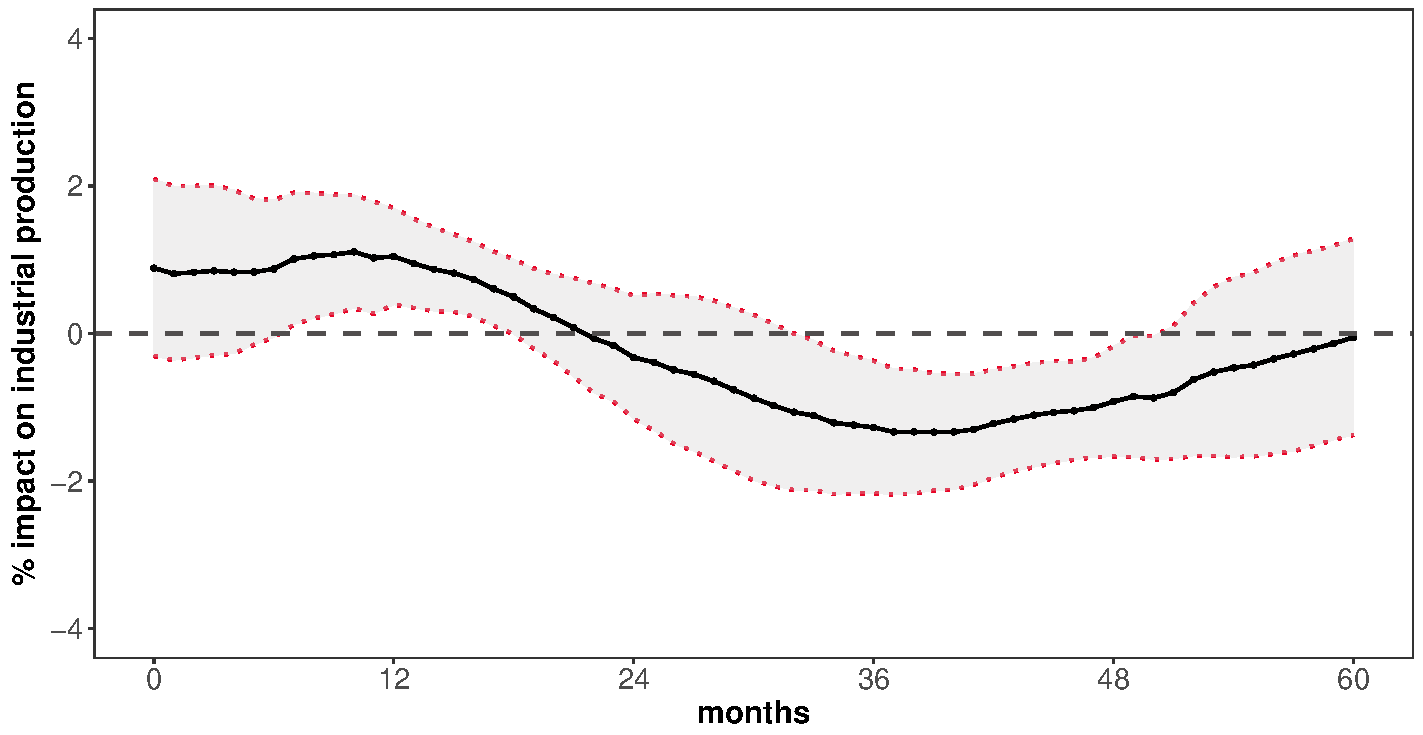
\includegraphics[trim=1cm -2.5cm 0.8cm -1cm, width=0.8\textwidth]{irf1.pdf}}
      \caption[Local projection estimations of the impact of a volatility shock on industrial production.]{Local projection estimations of the impact of a volatility shock on industrial production.
      \textit{Note:} Dashed lines are 1 standard-error bands around the response to a volatility shock.}
   \label{fig:irf1}
\end{figure}


\begin{figure}[!h]
   \centering
   \setlength\fboxsep{0pt}
   \setlength\fboxrule{0pt}
   \fbox{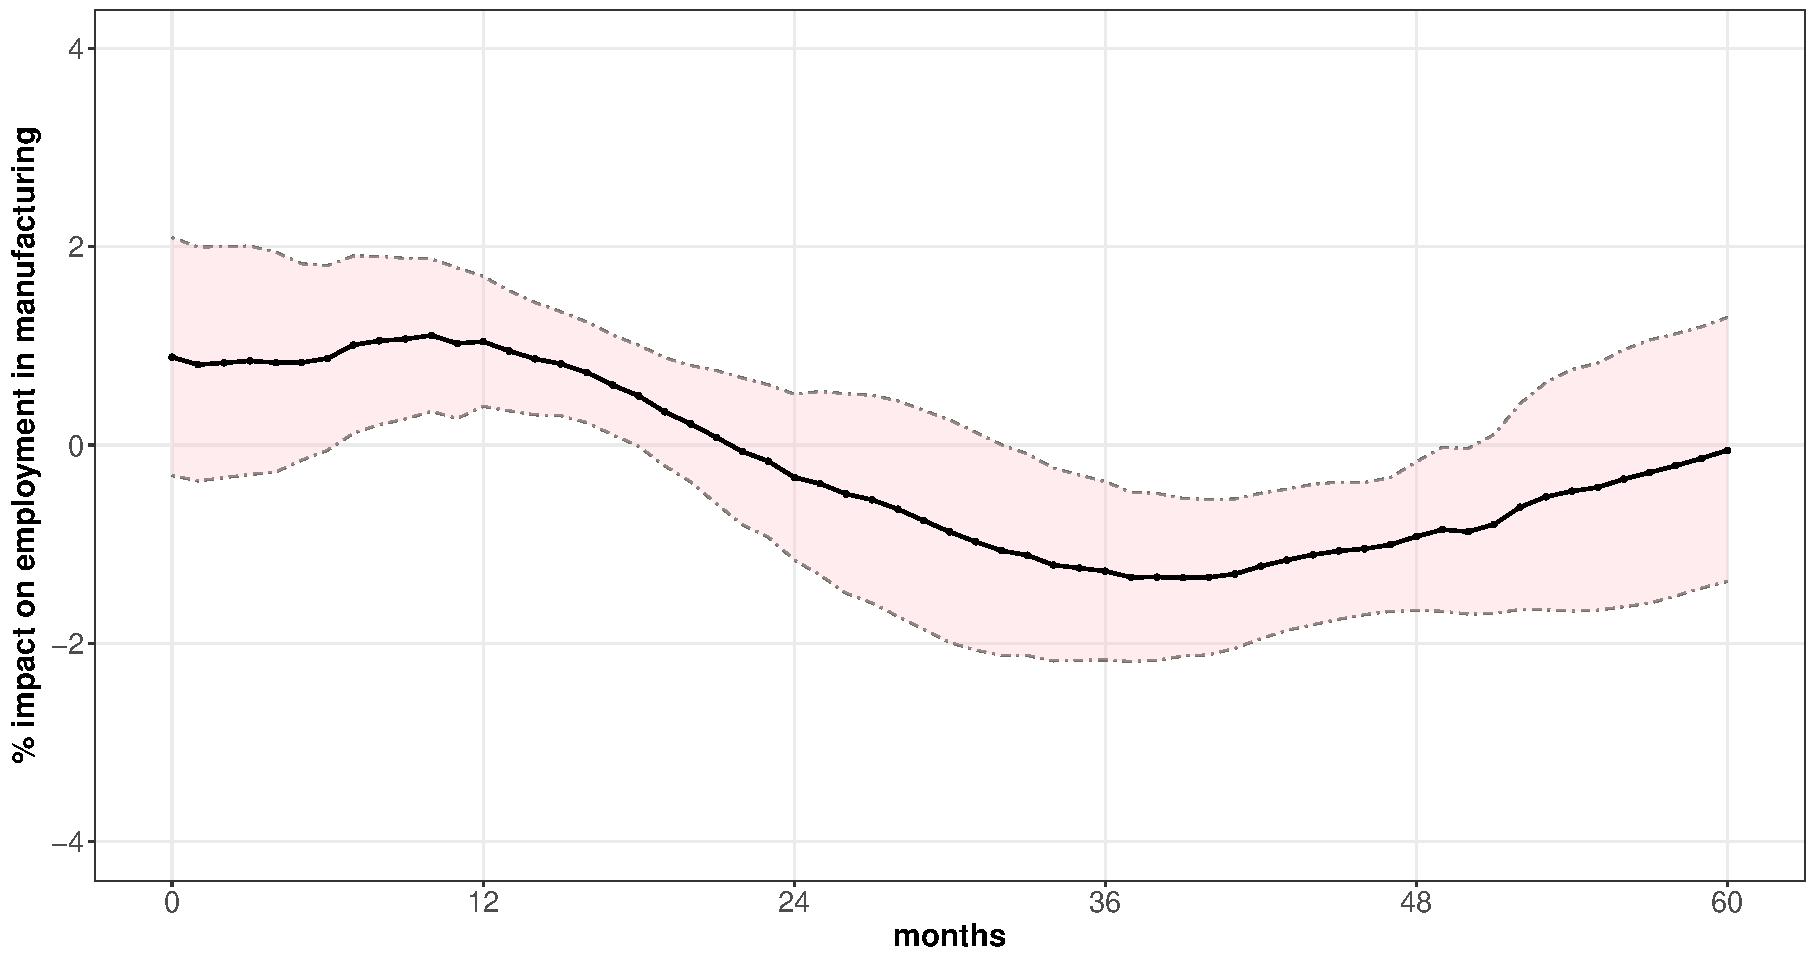
\includegraphics[trim=1cm -2.5cm 0.8cm -1cm, width=0.8\textwidth]{irf2.pdf}}
      \caption[Local projection estimations of the impact of a volatility shock on employment in manufacturing.]{Local projection estimations of the impact of a volatility shock on industrial production.
      \textit{Note:} Dashed lines are 1 standard-error bands around the response to a volatility shock.}
   \label{fig:irf2}
\end{figure}


\begingroup
    \fontsize{8pt}{12pt}\selectfont
    Note to self:
\begin{itemize}  
	\item ``Real GDP has the virtue of being the broadest indicator of real economic activity. Its downside is that it is difficult to measure [...]. For this reason, we also consider two other indicators: industrial production and the unemployment rate. Industrial production has the benefit of being relatively straightforward to measure; unemployment has the benefit of being perhaps the closest to a purely cyclical indicator.'' (Romer \& Romer, p. 3092)
	\item Footnote 17 in \citet{romandrom:17}: ``The impulse response functions in Figure 4 are estimated using the Jordà local projection method. Figure C2 of online Appendix C shows that the results estimated using a conventional vector autoregression are virtually identical.'' --> should we include a comparison with Bloom's VAR?
	\item \citet[p. 3096]{romandrom:17}: ``To do this, we run the same regression as in equation (1), but with our new measure of financial distress as the dependent variable. Since by construction the response of distress to itself is one at t = 0, we only estimate the regression for horizons 1 to 10. This analysis shows that distress is very serially correlated, particularly at near horizons. This finding suggests that some of the near-term persistence we find in the negative aftermath of financial distress is likely due to persistence in distress itself. It is not necessarily that financial crises have long-lasting effects, but rather that crises themselves tend to last for a while. This possibility [...] is analyzed further in Section III.''
	\item \citet[p. 3097]{romandrom:17}: ``Given that our new series on financial distress differs in important ways from existing crisis chronologies, it is useful to compare our findings for the average aftermath of financial crises with those estimated using the other series.'' --> We can use this approach similarly by using various uncertainty measures in our regressions as alternative and compare the impulse-response functions.
	\item \citet[p. 3099]{romandrom:17}, \textit{Dealing with Heteroskedasticity}: ``The first issue is possible differences in the variance of the residuals across countries. Economic activity is typically much more volatile in the less developed countries in our sample (such as Greece and Turkey), and in the smaller countries. It is plausible to think that the variances of the residuals in equation (1) also vary systematically by country. \\
	--> Taking into account heteroskedasticity in the residuals has a substantial impact on the estimates. Though the time pattern of the decline in GDP is relatively unchanged, the maximum decline is reduced by about one-third.''
	\item \citet[p. 3010]{romandrom:17}: ``In a related exercise, we also consider alternatives to conventional standard errors. In addition to heteroskedasticity of the residuals, there may also be serial correlation due to the overlapping structure of the residuals. We therefore experiment with both heteroskedasticity-consistent standard errors, and two forms of heteroskedasticity- and serial-correlation-corrected standard errors. Table C1 of online Appendix C shows that the alternative standard errors are typically about 30 to 50 percent larger than conventional standard errors. Thus, using the alternatives reduces the statistical significance of the estimated negative aftermath of a financial crisis substantially. Nonetheless, the estimates for GDP remain statistically significant at standard levels at all horizons.''
	\item \citet[p. 15]{ramzub:18}: ``The only complication associated with the Jordà method is the serial correlation in the error terms induced by the successive leading of the dependent variable. Thus, we use the Newey-West correction for our standard errors \citep{newest:87}.''
	\item \citet[p. 16]{ramzub:18}: ``Later, we will be comparing our baseline estimated to those from a threshold VAR." (--> This is something that we can maybe do as well; see a comment added above already!)
	\item \citet[p. 23]{ramzub:18}, footnote 20: ``We only estimate multipliers out five years because the Jordà method is less reliable at long horizons.''
	\item When it comes to describing the data sources I should have a look at the way how \citet{ramzub:18} explain each series in the Appendix.
	\item \citet[p. 17]{ramey:16}: ``If the VAR adequately captures the data generating process, this method is optimal at all horizons. If the VAR is misspecified, however, then the specification errors will be compounded at each horizon. To address this problem, Jordà (2005) introduced a \textit{local projection} method for estimating impulse responses.''
	\item \citet[p. 18]{ramey:16}: ``The control variables need not include the other $Y's$ as long as $\epsilon_{1t}$ is exogenous to those other $Y$'s. Typically, the control variables include deterministic terms (constant, time trends), lags of the $Y_i$, and lags of other variables that are necessary to "mop up''; \\
	One estimates a separate regression for each horizon and the control variables do not necessarily need to be the same for each regression. Note that except for horizon $h=0$, the error term $\xi_{t+h}$ will be serially correlated because it will be a moving average of the forecast errors from $t$ to $t+h$. Thus, the standard errors need to incorporate corrections for serial correlation, such as a \citep{newest:87} correction.
	\item \citet[p. 37]{ramey:16}: The term ``troughs'' is very often used in the context of impulse response functions. Here an example sentence: ``Industrial production begins to fall in the next month and roughs 21 months later.'' Literally translated it means "tief fallen" (auf sein tiefstes Niveau fallen).\\
	Another interesting expression is used on p. 39: ``[...] until they bottom out during the fourth year after the shock.''
	\item \citet[p. 45]{ramey:16}: ``Why does the Jordà method give such different estimates from the proxy SVAR?'' --> This is a question that I could actually elaborate on to possibly also compare our results investigating uncertainty using the Jordà method as opposed to the VAR that Bloom uses in his paper.
	\item In the presentation on the following web-page \url{http://www.datavis.ca/courses/RGraphics/R-Graphics1.pdf} on p. 35 I found an interesting way of plotting regression estimates! (instead of tables with standard errors, we plot the coefficients and confidence bands which let's the viewer immediately understand whether a coefficient is significantly different from zero or not.
\end{itemize}
\endgroup




\subsection{Robustness Checks: Alternative Uncertainty Measures}
This part provides results from a large number of robustness exercises designed to check the sensitivity of our results to various assumptions. (this sentence is formulated like this by \citet{juradoetal:15}).

\subsection{Interpretation of Results}
\begingroup
    \fontsize{8pt}{12pt}\selectfont
    Note to self:
\begin{itemize}
	\item \citet[p. 1181]{juradoetal:15} write: ``While we find that increases in uncertainty are associated with large declines in real activity, we caution that our results are silent on wehther uncertainty is the cause or effect of such declines. Our goal is to develop a defensible measure of time-varying macro uncertainty that can be tracked over time and related to fluctuations in real activity and asset markets. Our estimates do, however, imply that the economy is objectively less predictable in recessions thatn it is in normal times. This result is not a statement about changing subjective perceptions of uncertainty in recessions as compared to booms. Any theory for which uncertainty is entirely the effect of recessions would need to be consistent with these basic findings.  
\end{itemize}
\endgroup

%\newpage
\chapter{Conclusion}
\label{Conclusion}




%%%%%%%%%%%%%%%%%%AB HIER ENDET DER INHALT DER ARBEIT%%%%%%%%%%%%%%%%%%%
%%%%%%%%%%%%%%%%%%AB HIER ENDET DER INHALT DER ARBEIT%%%%%%%%%%%%%%%%%%%
%%%%%%%%%%%%%%%%%%AB HIER ENDET DER INHALT DER ARBEIT%%%%%%%%%%%%%%%%%%%
\newpage
\appendix

\chapter{Appendix}
\label{DataAndCode}
\section{Data: Sources and Description}
\label{sec:data}


Table with all the series used (using an internal numbering)



No.	Short Name	Source			Code			Tran 		Description
1	IP: mfg		IHS Global Insights	M_116461013		deltaln	Industrial Production Index - Manufacturing
IP_MAN: Industrial Production: Manufacturing (NAICS) (Board of Governors) Obtained via FRED (series name: IPMAN)

(note: I have, for now, downloaded the data from FRED; therefore my numbers are slightly different!)
2	Emp: mfg		IHS Global Insights	M_123109542		deltaln	Employees on Nonfarm PAyrolls: manufacturing
EMP_MAN: AAll Employees: Manufacturing, SA (BLS) Obtained via FRED (series name: MANEMP)

3	Avg hrs: mfg	IHS Global Insights	M_14386098		deltaln	Average Weekly Hours of Production and Nonsupervisory Workers: manufacturing
HOURS_MAN: Average Weekly Hours of Production and Nonsupervisory Emploees: Manufacturing, SA (BLS)
Obtained via FRED (series name: AWHMAN)

4	CPI-U: all		IHS Global Insights	M_110157323		delta^2 ln	CPI-U: all items
CPI: Consumer Price Index for All Urban Consumers: All Items (BLS) Obtained via FRED (series name: CPIAUSCL)

5	AHE: mfg		IHS Global Insights	M_123109552		delta^2 ln	Avg Hourly Earnings of PRod or Nonsup Workers Private Nonfarm - Manufacturing
EARN_MAN: Average Hourly Earnings of Production and Nonsupervisory Employees: Manufacturing, SA (BLS)
Obtained via FRED (series name: AHEMAN)

6	Fed Funds	IHS Global Insights	M_110155157		deltalv	Interest Rate: Federal Funds
FEDFUNDS: Loga Effective Federal Funds Rate, NSA (Boar dof Governors) Obtained via FRED (series name: FEDFUNDS)

7	S\&P 500		IHS Global Insights	M_110155044		deltaln	S\&P's Common Stock Price Index: Composite
												





Then we create separate explanations about which variables were used for which model:

for VAR-8 estimations (following \citet{bloom:09}
Industrial Production Index (IP): manufacturing --> Source: IHS Global Insights

for VAR-11 estimations (following \citet{bloom:09}


\newgeometry{left=25mm, right=25mm, top=30mm, bottom=30mm}
%the below code is to adjust the header ruler after the
%newgeometry!
\fancyhfoffset[E,O]{0pt}
\section{Code}
\label{sec:rcode}
%\begin{Verbatim}[fontsize=\small]
%halloe
%\end{Verbatim} 

%\begin{verbatim}
%halloe
%\end{verbatim} 

\begingroup
\fontsize{9pt}{12pt}\selectfont
\begin{verbatim}  
##The Code will go here.









\end{verbatim}  
\endgroup


\restoregeometry
\chapter{Appendix}
\label{VARAndLocalProjection}
\section{IRFs in a VAR-Setting}
\section{IRFs and Local Projections}

%%%%%%%%%%%%%%%%%%%%%%%%%BIBLIOGRAPHY%%%%%%%%%%%%%%%%%%%%%%%%%%%%
%%%%%%%%%%%%%%%%%%%%%%%%%BIBLIOGRAPHY%%%%%%%%%%%%%%%%%%%%%%%%%%%%
%%%%%%%%%%%%%%%%%%%%%%%%%BIBLIOGRAPHY%%%%%%%%%%%%%%%%%%%%%%%%%%%%

\nocite{*}
\clearpage
\thispagestyle{empty}
\bibliographystyle{agsm}
%bibliographystyle{agsm} bewirkt, dass KEINE Beistriche zwischen den Jahreszahlen sind. Dafür aber
%Gänsefüßchen beim Titel der Werke!
\bibliography{mybiblio}





%%%%%%%%%%%%%%%%%%%%%%EIDESSTATTLICHE ERKLÄRUNG%%%%%%%%%%%%%%%%%%%%%%
\clearpage
\thispagestyle{empty}
\null\vspace{46pt}
\paragraph{\large{Declaration of Authorship}}
\vspace{43pt}
I hereby declare that I prepared this master's thesis independently and that the thoughts taken
directly or indirectly from other sources are acknowledged as references accordingly. \\
\\
The work contained in this thesis has neither been previously submitted to any other examination authority nor published in any other form which has led to the award of a degree.\\[10mm]

    Innsbruck, \makebox[1.8in][l]{\hrulefill} \qquad \makebox[2.6in]{\hrulefill}\\
    \makebox[2.95in][l]      \hfill\makebox[2.0in][l]{(Signature: Marcel Kropp)}



%%%%%%%%%%%%%%%%%%%%%%EIDESSTATTLICHE ERKLÄRUNG%%%%%%%%%%%%%%%%%%%%%%

\end{document}
%%%%%%%%%%%%%%%%%%%%%%END OF THE DOCUMENT%%%%%%%%%%%%%%%%%%%%%%%%%%
%%%%%%%%%%%%%%%%%%%%%%END OF THE DOCUMENT%%%%%%%%%%%%%%%%%%%%%%%%%%
%%%%%%%%%%%%%%%%%%%%%%END OF THE DOCUMENT%%%%%%%%%%%%%%%%%%%%%%%%%%